The summary of the systematic effects and components that they affect considered 
in the $\Hi \to\WW \to 2\ell2\nu$ analysis is shown in Table~\ref{tab:hwwsyst}. 
To simplify, the following convention names are used to identify several signal 
and background processes: ggH (for $gg \to H$), qqWW (for $qq \to \WW$), ggWW 
(for $gg \to\WW$), VV (for $\WZ$ plus $\Z\Z$), Top (for $\ttbar$ plus $\tw$), 
Zjets (for $\dymm$ plus $\dyee$), Wjets (for $\Wjets$), Wgamma (for $\W+\gamma$) 
and Ztt (for $\dytt$).

\begin{table}[!ht]
\begin{center}
{\small
\begin{tabular}{|l|cccccccccccc|}
\hline
 Systematic Effect & ZH  & WH & qqH& ggH& qqWW & ggWW & VV & Top & Zjets & Wjets & Wgamma & Ztt\\
\hline
Higgs Theory       & X   & X  & X  & X  & -    & -    & -  & -   & -	 & -	 & -	  & - \\
PDF                & X   & X  & X  & X  & X    & X    & X  & -   & -	 & -	 & X	  & - \\
Lepton efficiency  & X   & X  & X  & X  & X    & X    & X  & X   & -	 & -	 & X	  & X \\
Lepton resolution  & X   & X  & X  & X  & X    & X    & X  & X   & -	 & -	 & X	  & X \\
MET resolution     & X   & X  & X  & X  & X    & X    & X  & X   & -	 & -	 & X	  & X \\
Jet Energy Scale   & X   & X  & X  & X  & X    & X    & X  & X   & -	 & -	 & X	  & X \\
\WW{}              & -   & -  & -  & -  & X    & X    & -  & -   & -	 & -	 & -	  & - \\
Top                & -   & -  & -  & -  & -    & -    & -  & X   & -	 & -	 & -	  & - \\
\dyll{}            & -   & -  & -  & -  & -    & -    & -  & -   & X	 & -	 & -	  & - \\
\wjets{}           & -   & -  & -  & -  & -    & -    & -  & -   & -	 & X	 & -	  & - \\
$\W\gamma$         & -   & -  & -  & -  & -    & -    & -  & -   & -	 & -	 & X	  & - \\
\dytt{}            & -   & -  & -  & -  & -    & -    & -  & -   & -	 & -	 & -	  & X \\
statistics         & X   & X  & X  & X  & X    & X    & X  & X   & X	 & X	 & X	  & X \\
\hline
\end{tabular}
\caption{Summary of the systematic effects and components that they affect considered in the 
$\Hi \to\WW \to 2\ell2\nu$ analysis.}
\label{tab:hwwsyst}
}
\end{center}
\end{table}

\subsubsection{Higgs Theoretical Uncertainties}
The theoretical systematic uncertainties on the signal yield is factorized into 
the product of two components. The first component is the uncertainty on the 
fraction of events categorized into the different jet bins and the effect of 
migrations across jet bins. The second component is the uncertainty on the 
lepton acceptance and the selection efficiency of all other cuts. The major
effect by far comes from the uncertainty on the normalization and it has been
described in detailed in~\cite{hww_eps, hww_lp}, following the prescriptions from
the Higgs cross section Yellow 
Report~\cite{LHCHiggsCrossSectionWorkingGroup:2011ti}.

The procedure to take into account a possible variation 
on the final discriminant variable due to the QCD renormalization ($\mu_R$) 
and scale ($\mu_F$) is to reweight the $gg \to H$ component with different k-factor
distributions. Since the normalization effects have their own factors, only a
shape variation is allowed. We the the ``up" variation as 
$\mu_R = 0.5\mu$ and $\mu_F =2.0\mu$ and the ``down" variation as 
$\mu_R = 2.0\mu$ and $\mu_F =0.5\mu$, being $\mu$ the nominal scale value. 
An example of the effect of this uncertainty is shown in Figure~\ref{fig:ggHsyst}. 
It is possible to see that the differences among the default distribution and the 
variations are very small.

\begin{figure}[!htbp]
\begin{center}
\subfigure[]{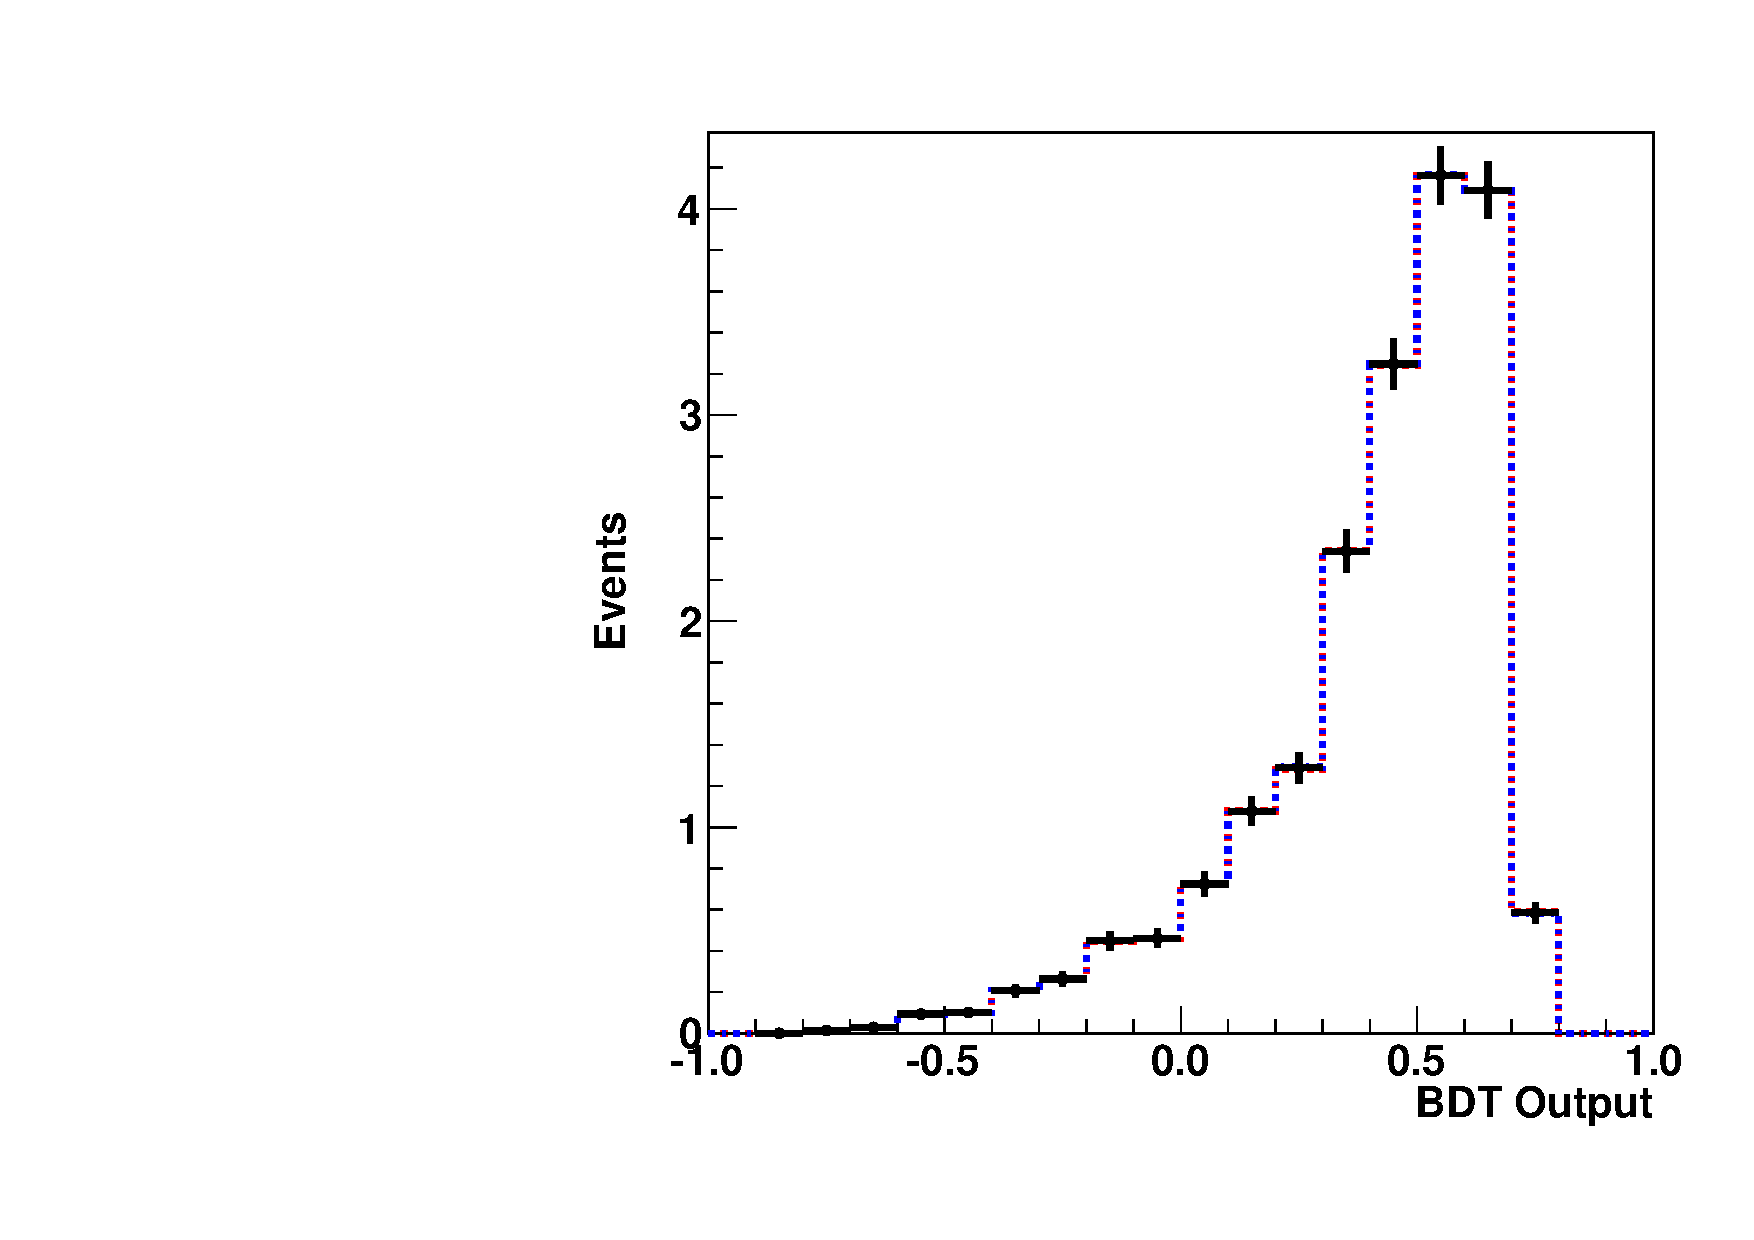
\includegraphics[width=0.49\textwidth]{figures/cvswwof_58.pdf}}
\subfigure[]{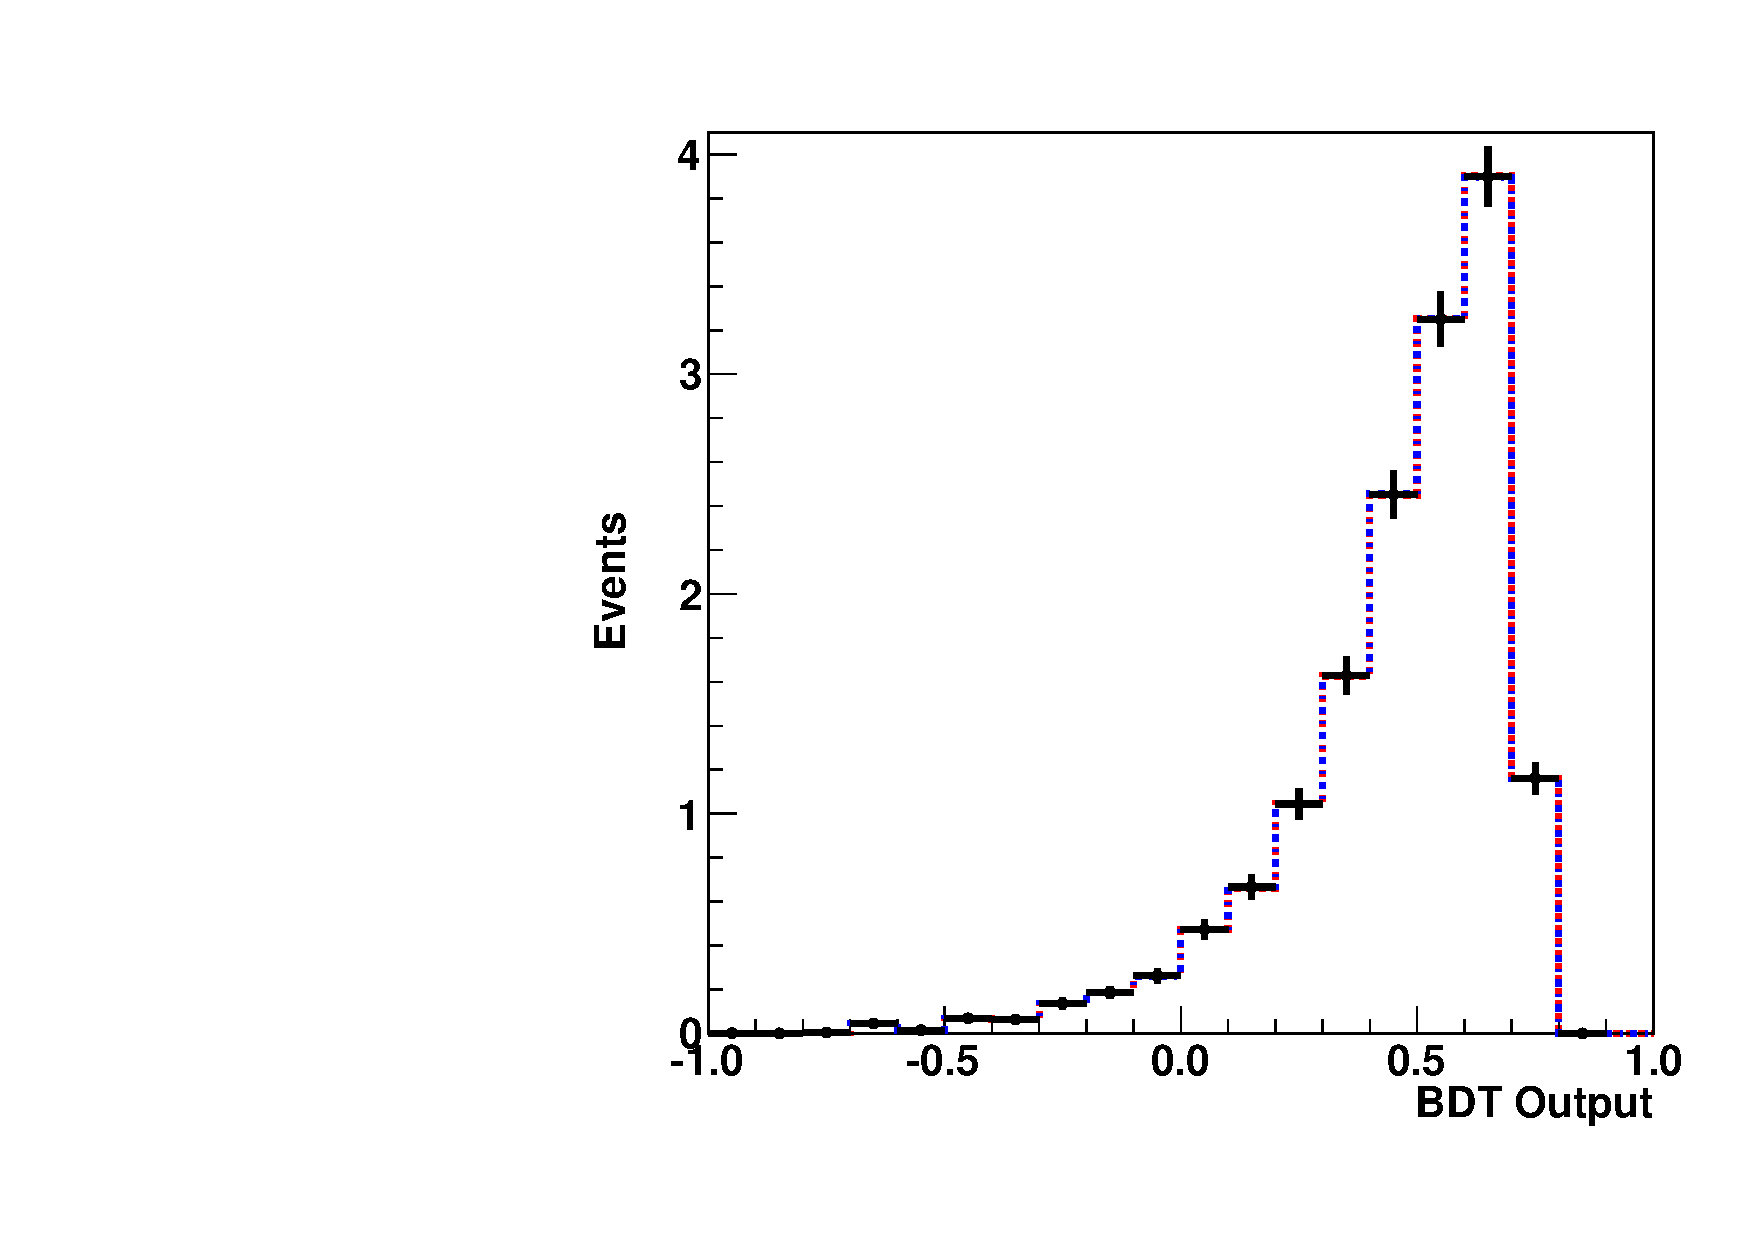
\includegraphics[width=0.49\textwidth]{figures/cvswwsf_58.pdf}}
\caption{BDT Output distribution for $H(130) \to \WW$ 0-jet bin analysis in $gg \to H$ events 
for $\mathcal{L}~=~1.55~\pm~0.07~\ifb$. Opposite-flavor (a) and same-flavor (b) final states 
are shown. The dots histogram is the default shape, while the dashed red histogram 
is the ``Up" component and the dashed blue histograms is the ``Down" component, for the 
theoretical uncertainties.}
\label{fig:ggHsyst}
\end{center}
\end{figure}

\subsubsection{Parton Distribution Functions}
Parton distribution functions (PDFs) are obtained from global fits 
to experimental data from deep in-elastic scattering, Drell-Yan, and jet 
processes. The recommendations of the PDF4LHC group were followed to obtain the
uncertainties due to the limited knowledge of such PDFs. From those studies~\cite{hww_eps, hww_lp}, 
we consider the overall normalisation uncertainty to adequately contain possible 
variations in the uncertainty as a function of the discriminant variable.

\subsubsection{Lepton Efficiency Scale Factors}
The lepton efficiencies are measured in data and simulated events using the 
well-known tag and probe method~\cite{hww_eps}, giving a scale factor to the
simulated events as a function of the $\pt$ and $\eta$ of each lepton. The
associated uncertainty may have some $\pt$ and $\eta$ dependence, leading to a
possible shape variation. The procedure to estimate the uncertainty due to the
lepton efficiency scale factor is to apply a $+1(-1)\sigma$ reweighting factor to the
lepton efficiency scale factor for the ``up" (``down") variation. Both
normalization and shape are considered with this procedure. 
An example of the effect of this uncertainty is shown in Figure~\ref{fig:qqWWeff}. 
It is possible to see that the differences among the default distribution and the 
variations are rather small.

\begin{figure}[!htbp]
\begin{center}
\subfigure[]{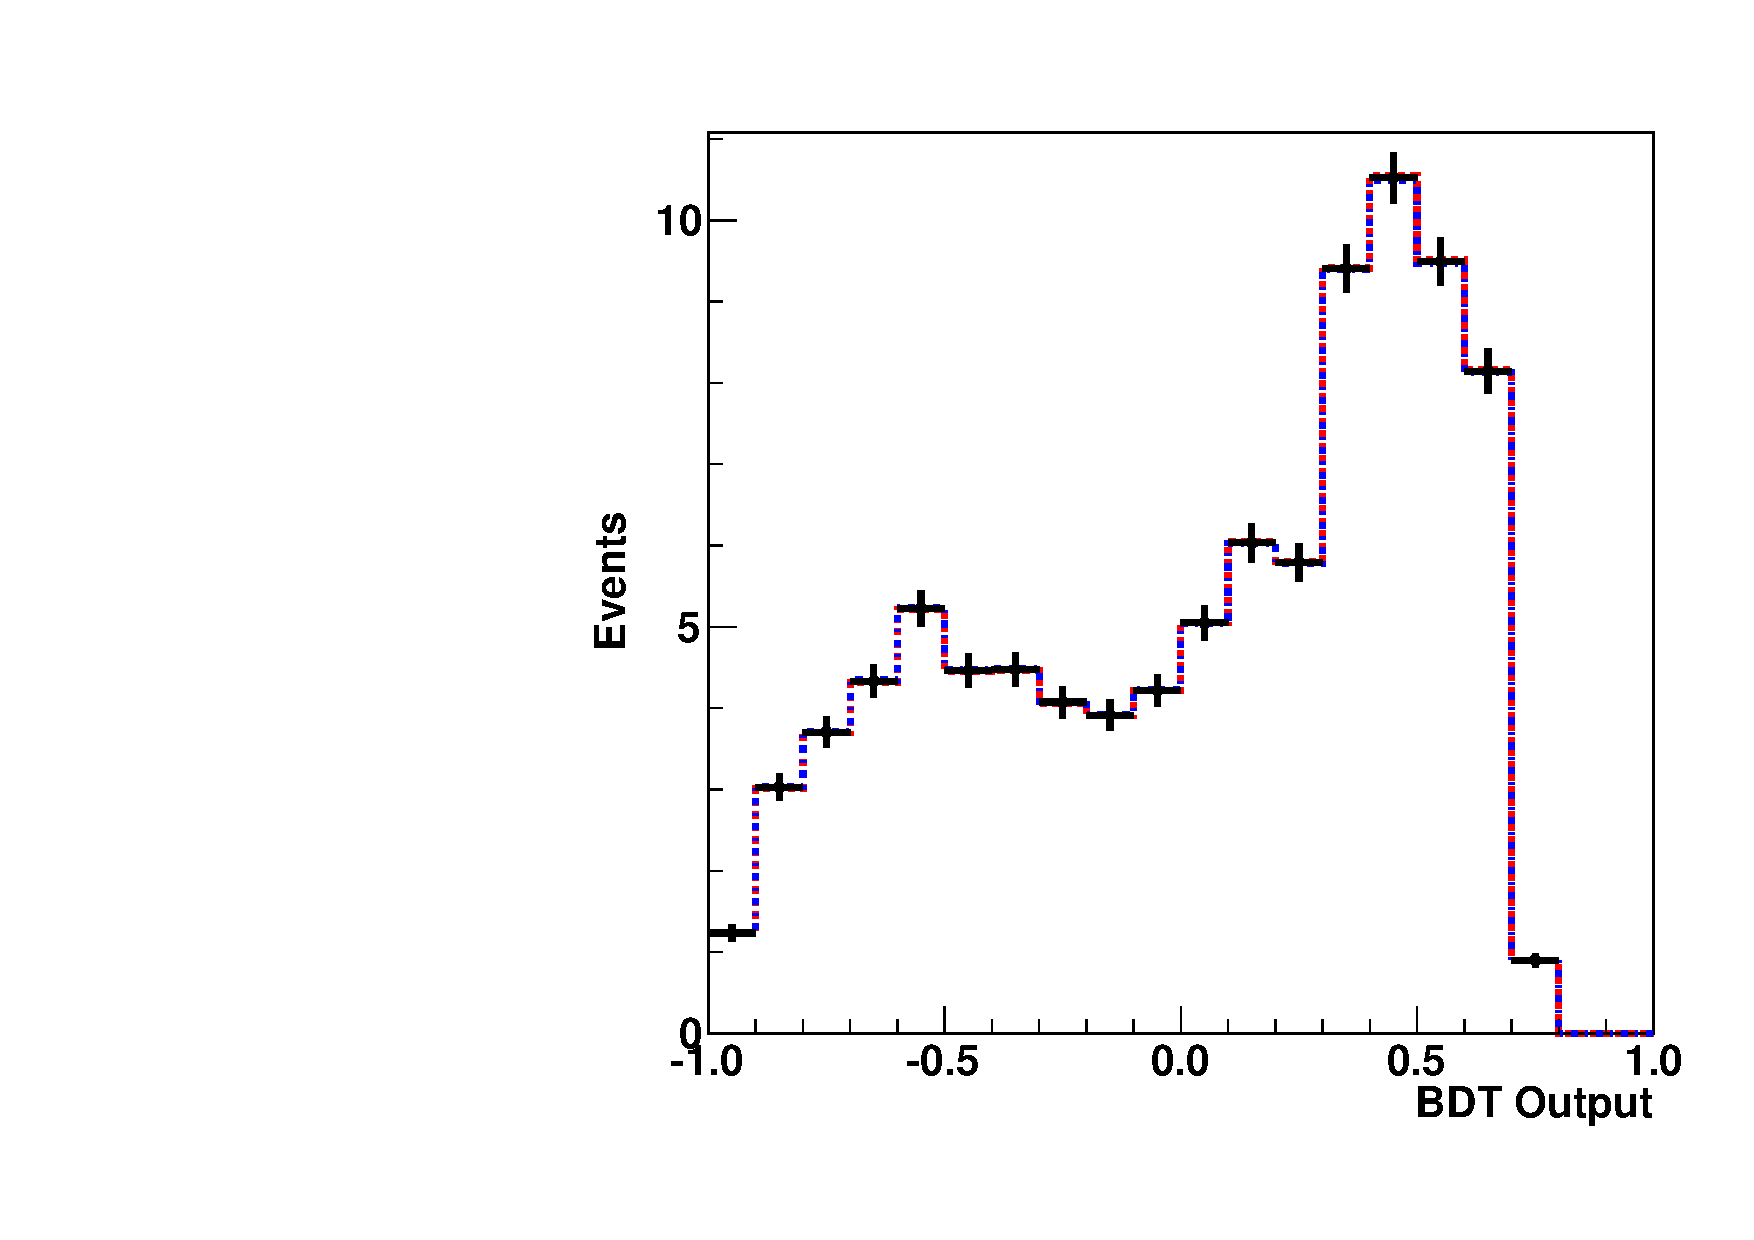
\includegraphics[width=0.49\textwidth]{figures/cvswwof_20.pdf}}
\subfigure[]{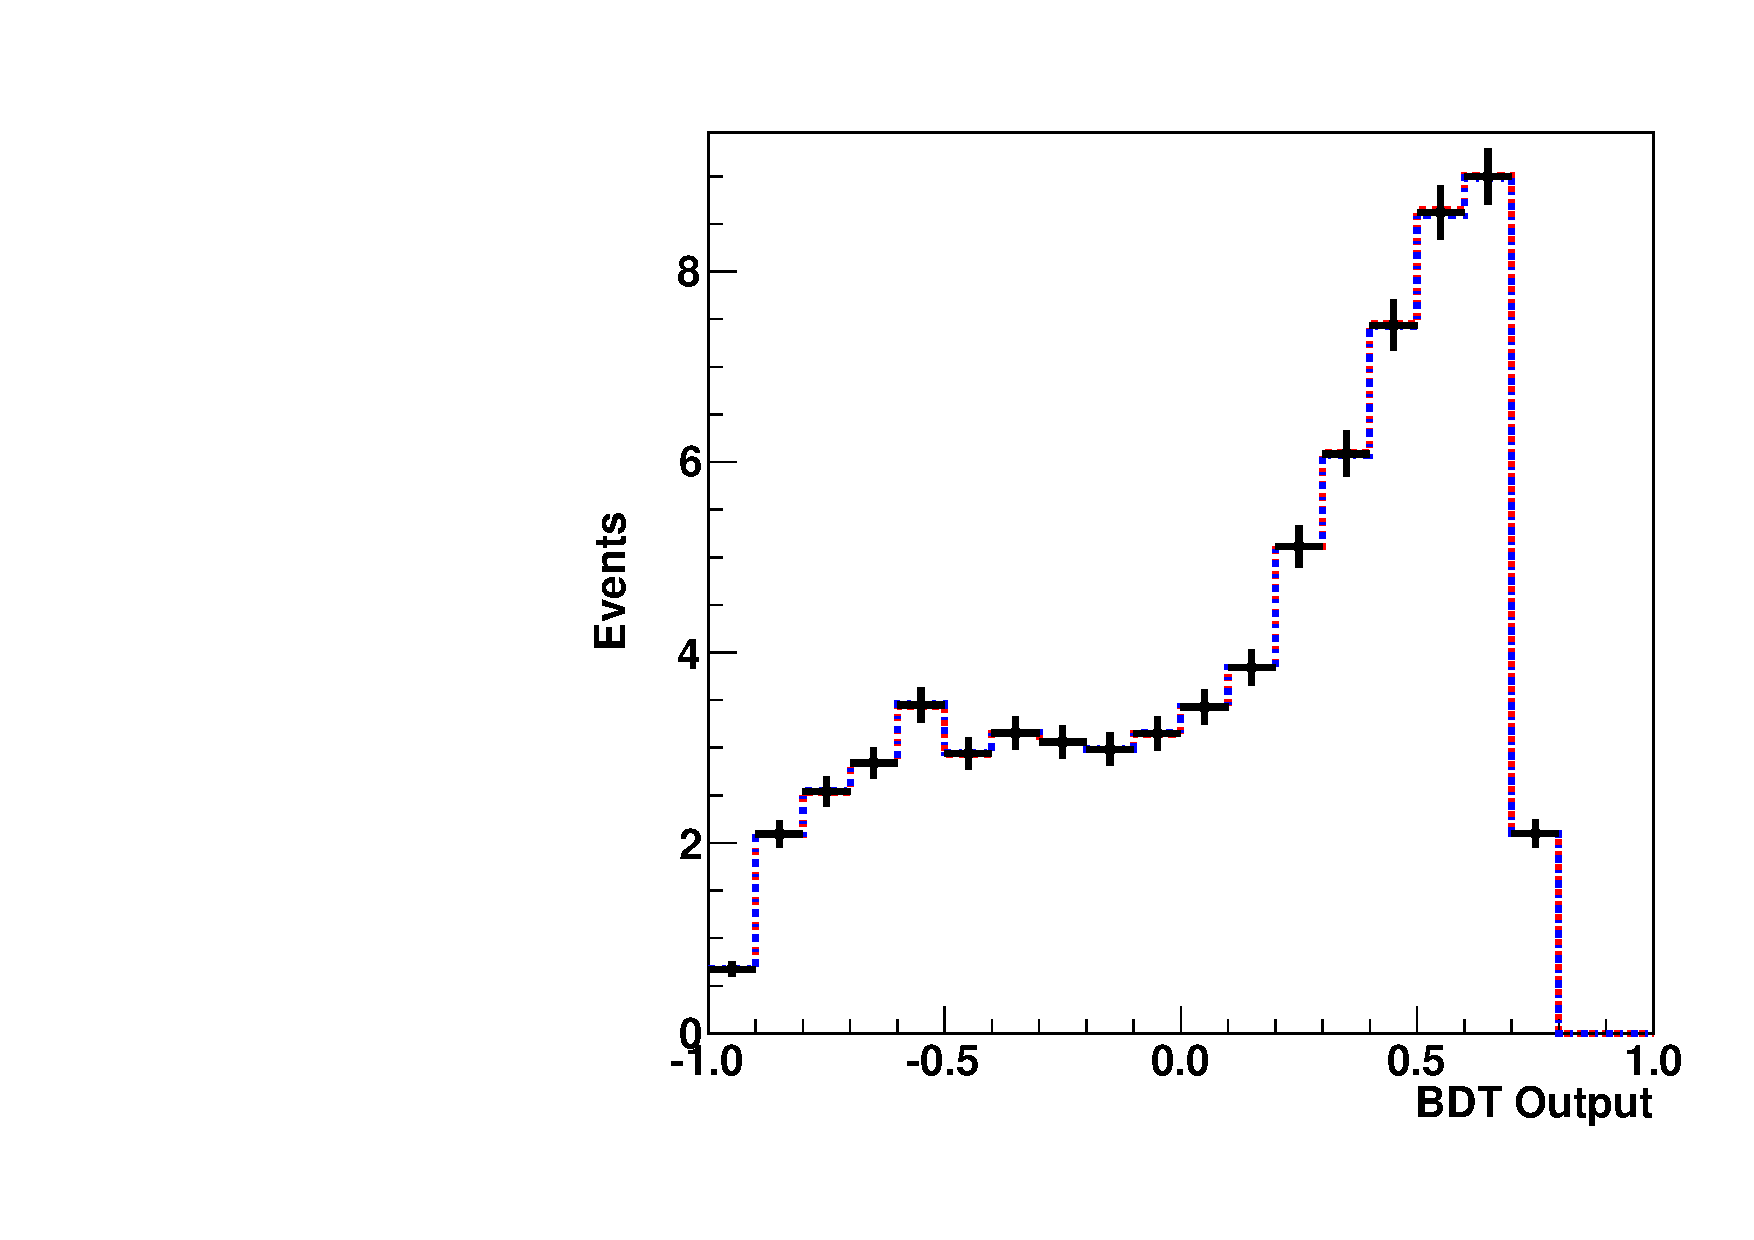
\includegraphics[width=0.49\textwidth]{figures/cvswwsf_20.pdf}}
\caption{BDT Output distribution for $H(130) \to \WW$ 0-jet bin analysis in $qq \to \WW$ events 
for $\mathcal{L}~=~1.55~\pm~0.07~\ifb$. Opposite-flavor (a) and same-flavor (b) final states 
are shown. The dots histogram is the default shape, while the dashed red histogram 
is the ``Up" component and the dashed blue histograms is the ``Down" component, for the 
lepton efficiency uncertainties.}
\label{fig:qqWWeff}
\end{center}
\end{figure}

\subsubsection{Lepton Energy-Momentum Resolution and Scale}
The lepton energy-momentum does not perfectly agree between data and simulated
events with the current available sample. To assign an uncertainty, we smear 
the lepton energy-momentum by a Gaussian with width equal to the central value 
determination of the resolution, and the central value the observed bias in
data. With the new four-momentum of both leptons, we build a new discriminant
variable. We take the ``up" (``down") variation as the positive (negative) biased
case. 
An example of the effect of this uncertainty is shown in Figure~\ref{fig:ggWWLepRes}. 

\begin{figure}[!htbp]
\begin{center}
\subfigure[]{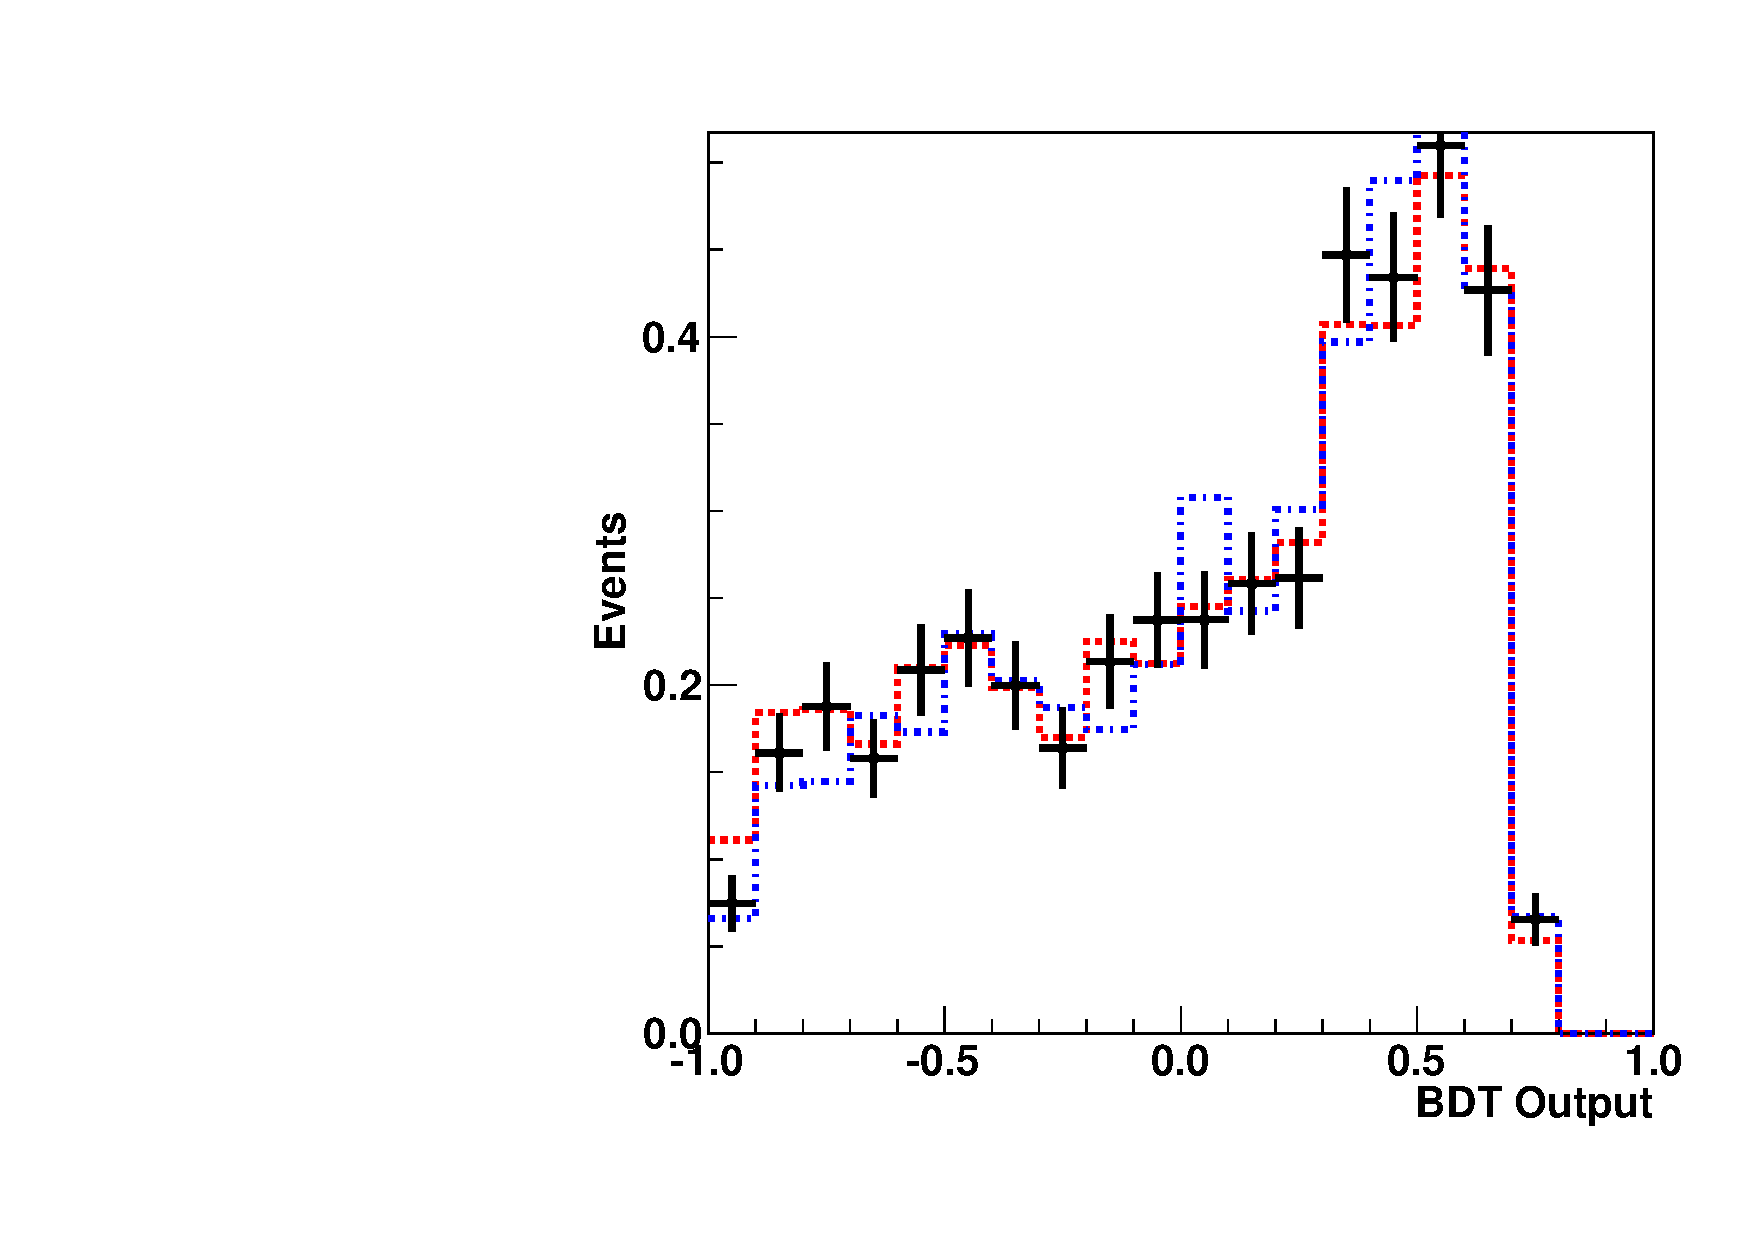
\includegraphics[width=0.49\textwidth]{figures/cvswwof_31.pdf}}
\subfigure[]{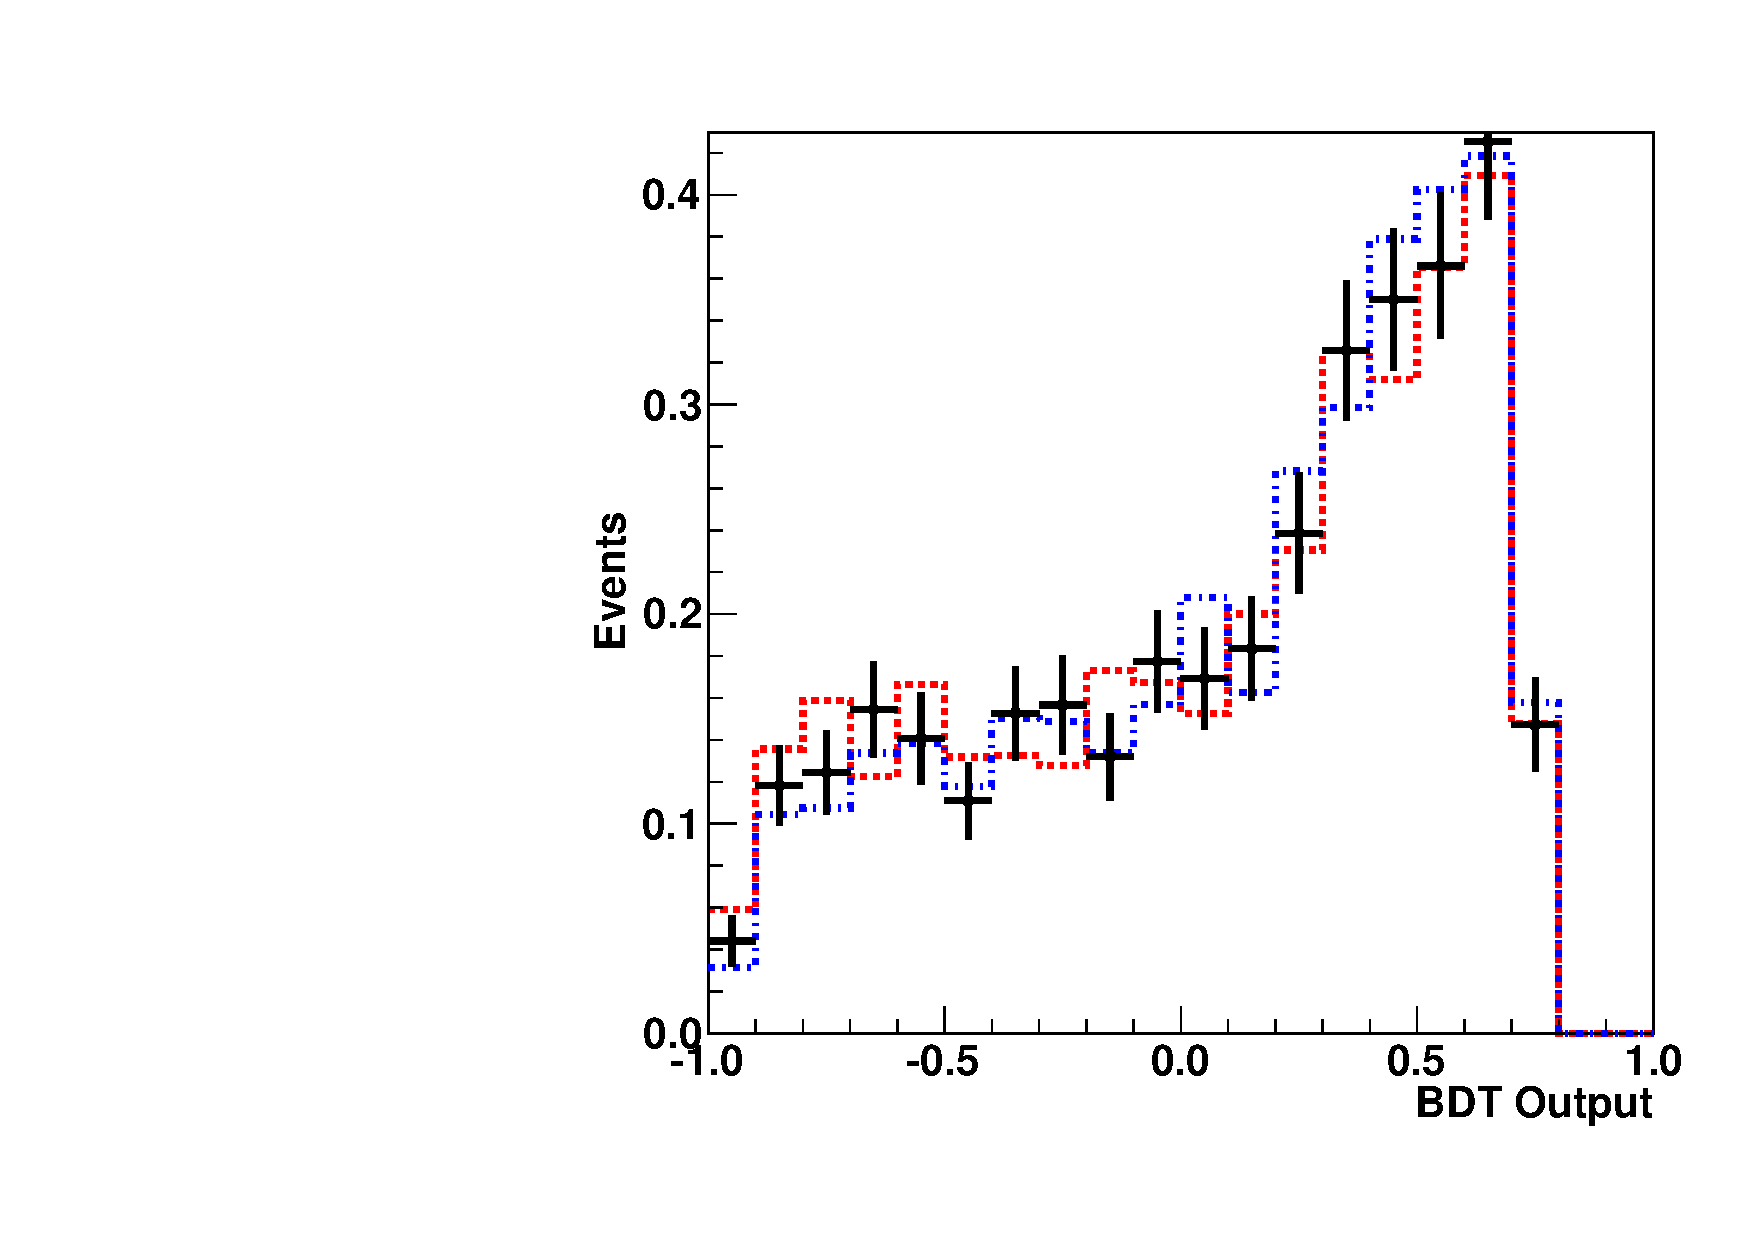
\includegraphics[width=0.49\textwidth]{figures/cvswwsf_31.pdf}}
\caption{BDT Output distribution for $H(130) \to \WW$ 0-jet bin analysis in $gg \to \WW$ events 
for $\mathcal{L}~=~1.55~\pm~0.07~\ifb$. Opposite-flavor (a) and same-flavor (b) final states 
are shown. The dots histogram is the default shape, while the dashed red histogram 
is the ``Up" component and the dashed blue histograms is the ``Down" component, for the 
lepton momentum resolution and scale uncertainties.}
\label{fig:ggWWLepRes}
\end{center}
\end{figure}

\subsubsection{$\met$ Resolution}
The $\met$ resolution in data is not well reproduced in simulated events leading
to an underestimation of $\dyll$ events, where no real $\met$ from neutrinos is
present. The background estimation from Zjets events has its own uncertainty.
Nevertheless, other processes with neutrinos in the final state may have an
uncertainty due to this effect. To account for it, we have smeared the X and Y
components of both $\met$ and $track-\met$ and produced new discriminant
variables with the smeared quantities. The smeared variable is the ``up"
variation, while we take the ``down" variation as the mirror of the difference
between the ``up" and default variables. 
An example of the effect of this uncertainty is shown in Figure~\ref{fig:VVMetRes}. 

\begin{figure}[!htbp]
\begin{center}
\subfigure[]{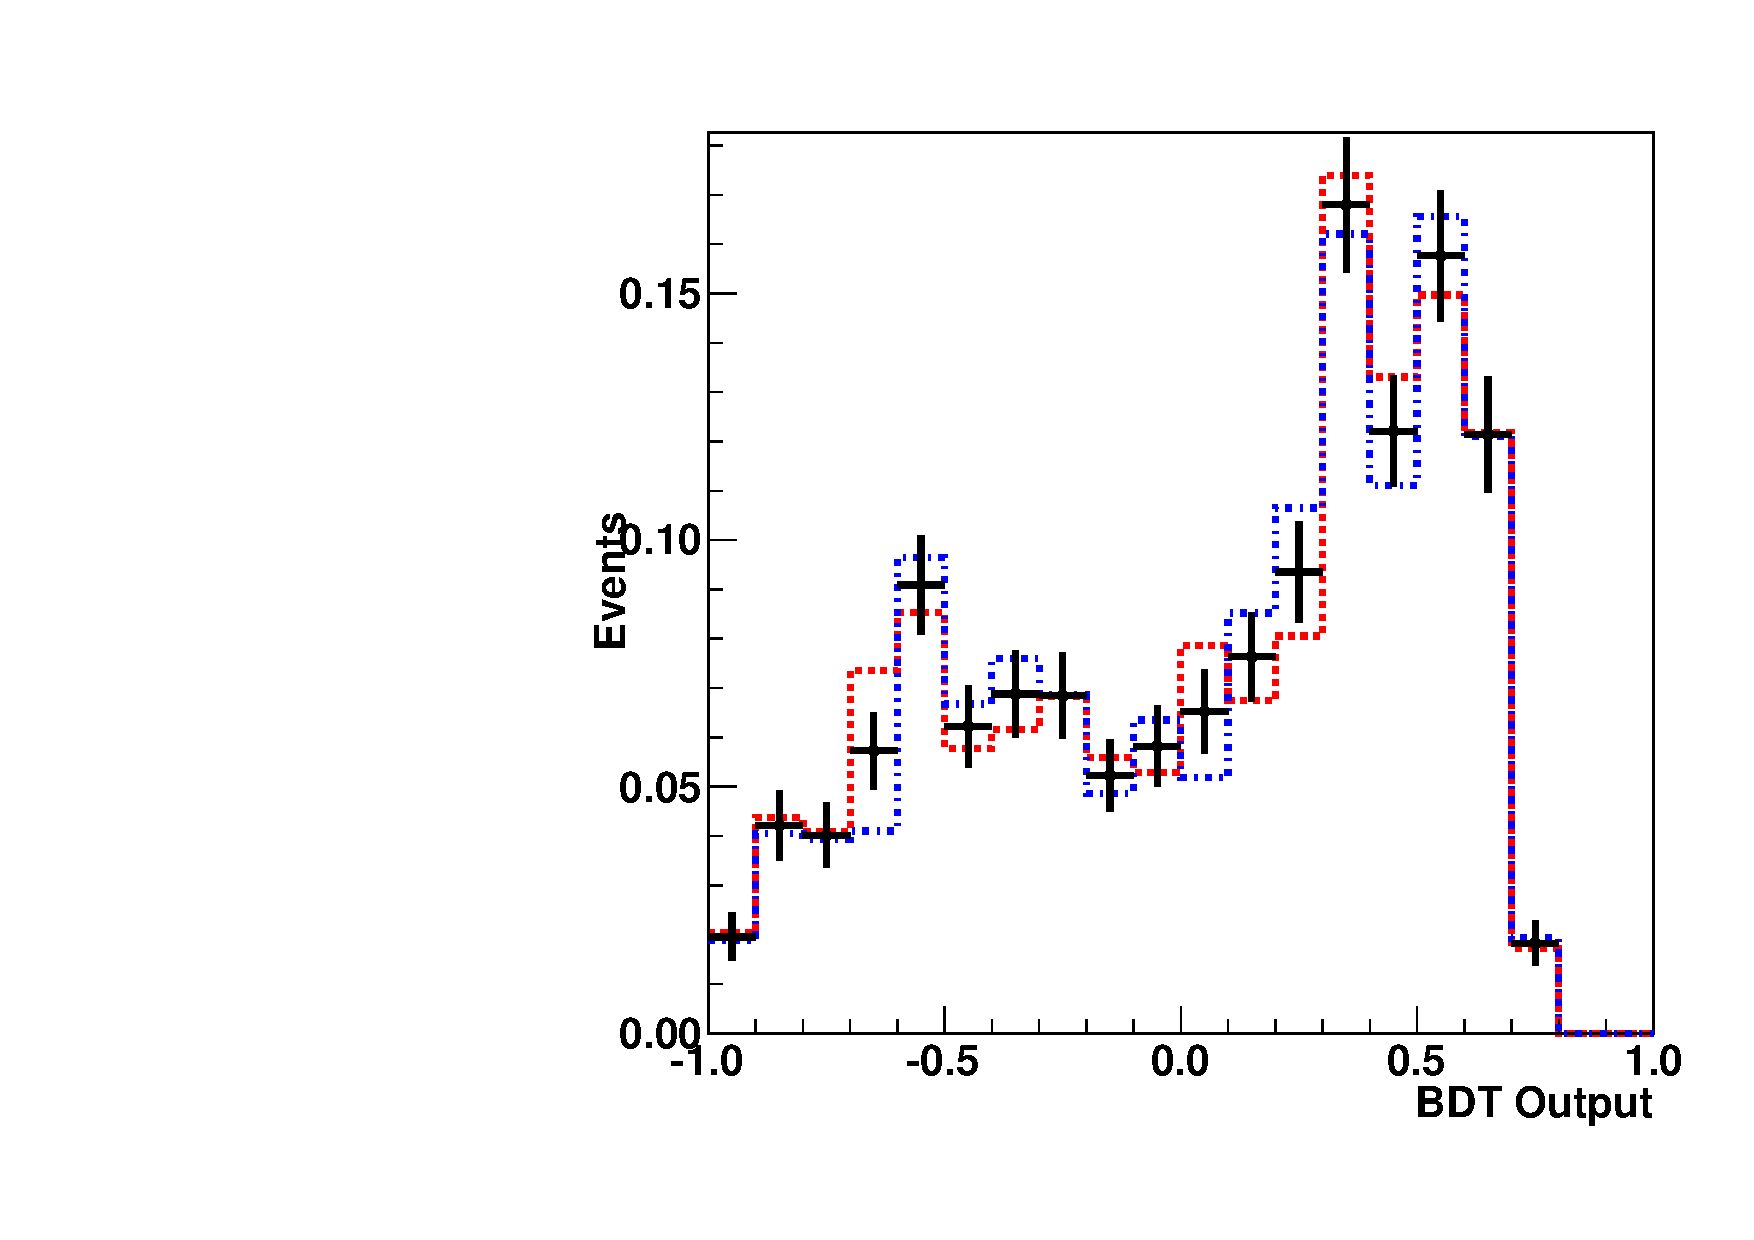
\includegraphics[width=0.49\textwidth]{figures/cvswwof_43.pdf}}
\subfigure[]{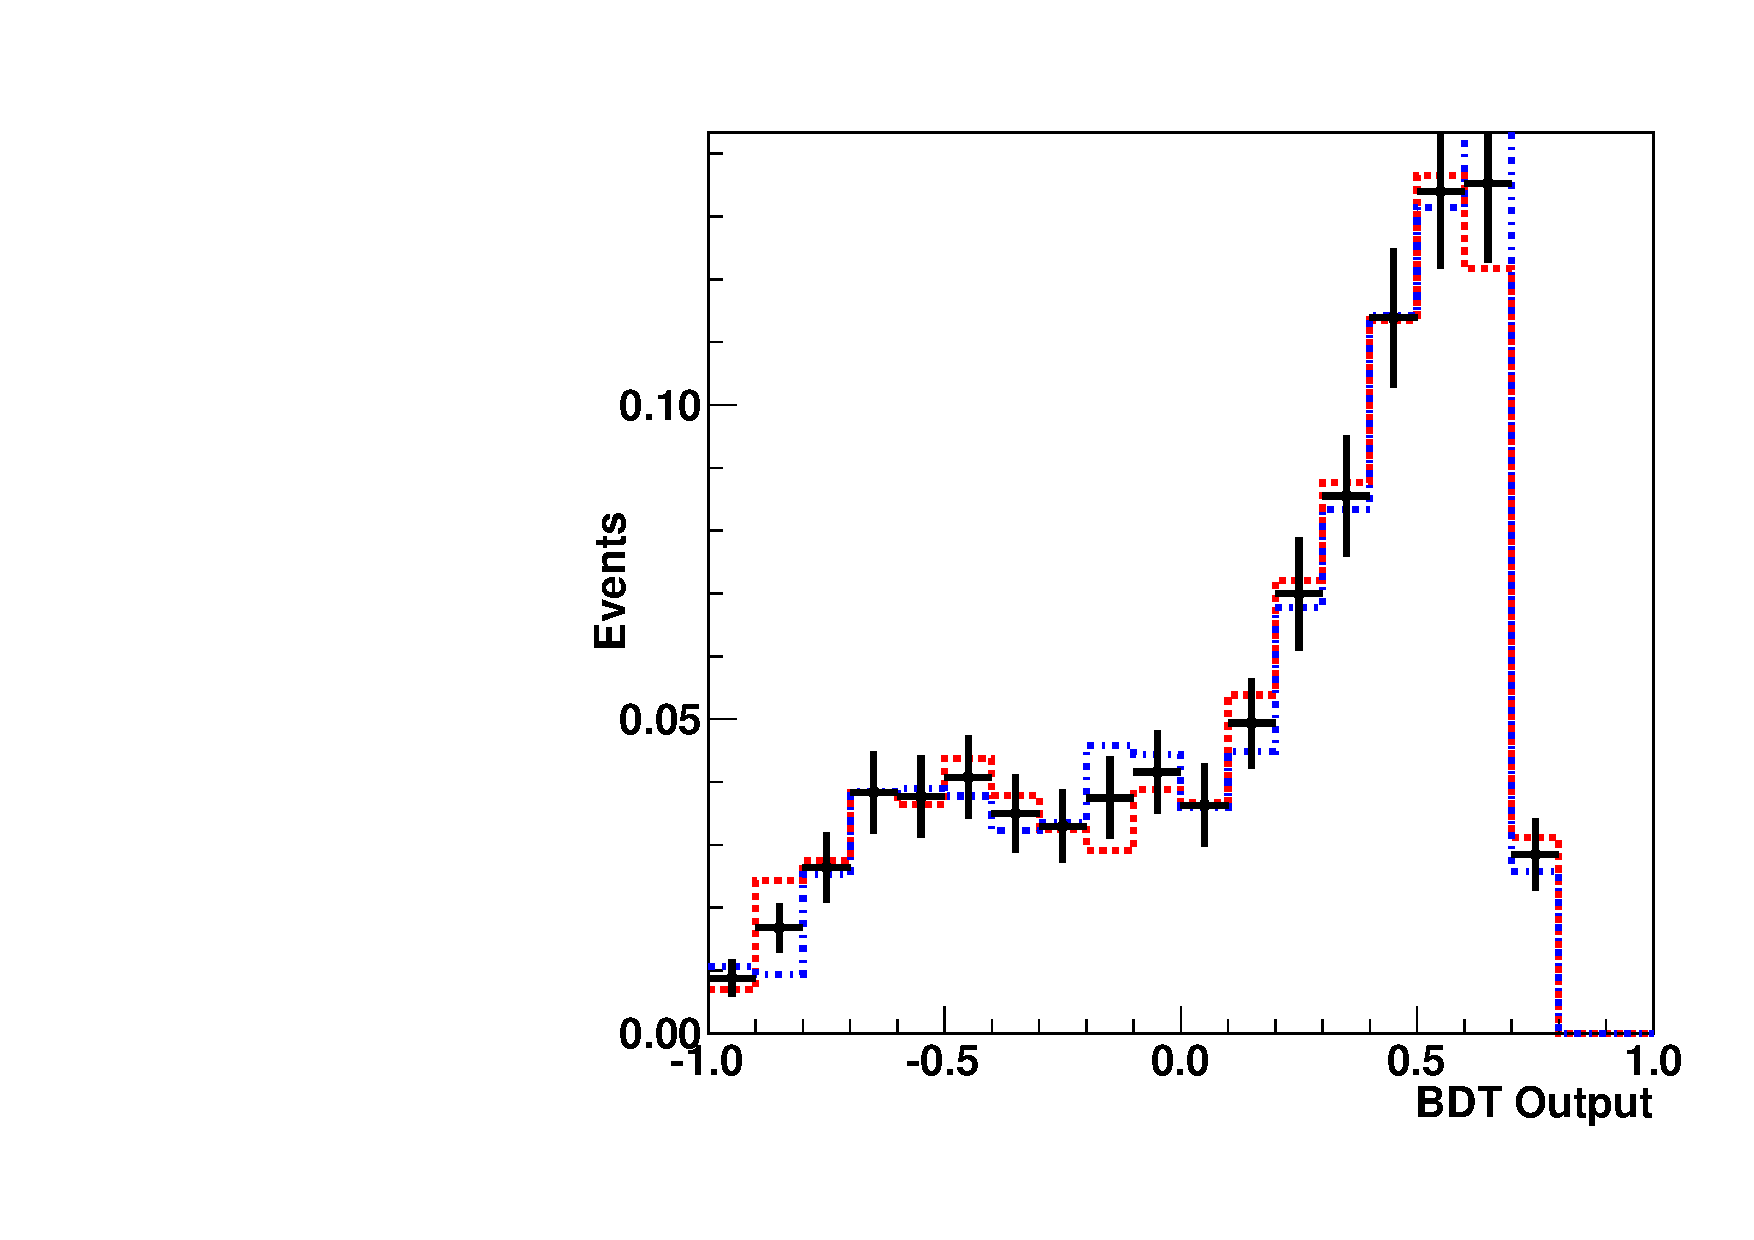
\includegraphics[width=0.49\textwidth]{figures/cvswwsf_43.pdf}}
\caption{BDT Output distribution for $H(130) \to \WW$ 0-jet bin analysis in $\WZ/\Z\Z$ events 
for $\mathcal{L}~=~1.55~\pm~0.07~\ifb$. Opposite-flavor (a) and same-flavor (b) final states 
are shown. The dots histogram is the default shape, while the dashed red histogram 
is the ``Up" component and the dashed blue histograms is the ``Down" component, for the 
$\met$ uncertainties.}
\label{fig:VVMetRes}
\end{center}
\end{figure}

\subsubsection{Jet Energy Scale}
The discriminant variables make no use of the jet energy quantities, therefore
there is no direct effect on the jet energy scale (JES) uncertainty, in addition
to the normalization uncertainty due to the migration among the different jet
bins. Nevertheless, it is observed that kinematic variables show different
distributions depending on the jet multiplicity. To assign an uncertainty,
we vary the transverse momentum of the jets by $\pm 5\%$ (``up" and ``down",
respectively) and build the new discriminant variables. Only shape uncertainties are 
considered in this case. 
An example of the effect of this uncertainty is shown in Figure~\ref{fig:ggHJES}. 
It is possible to see that the differences among the default distribution and the 
variations are rather small.

\begin{figure}[!htbp]
\begin{center}
\subfigure[]{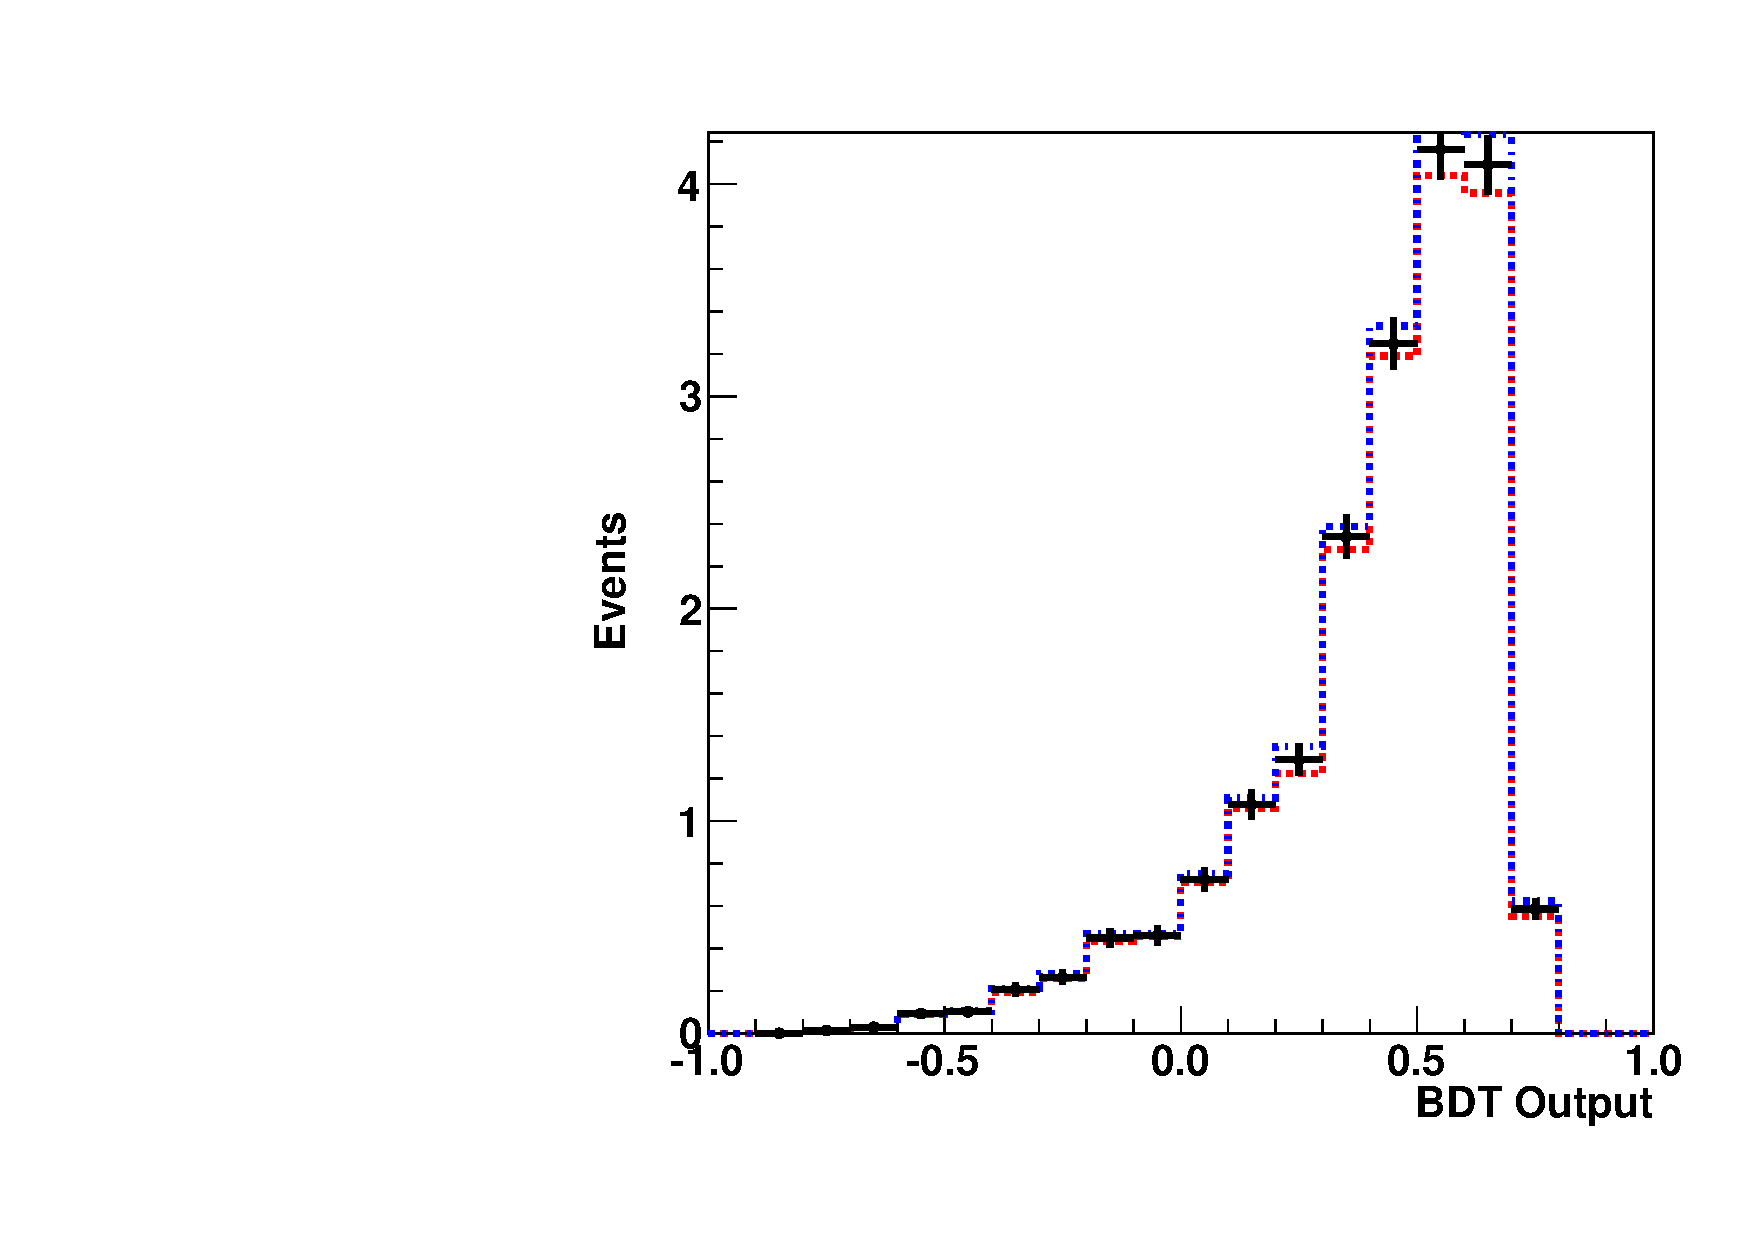
\includegraphics[width=0.49\textwidth]{figures/cvswwof_50.pdf}}
\subfigure[]{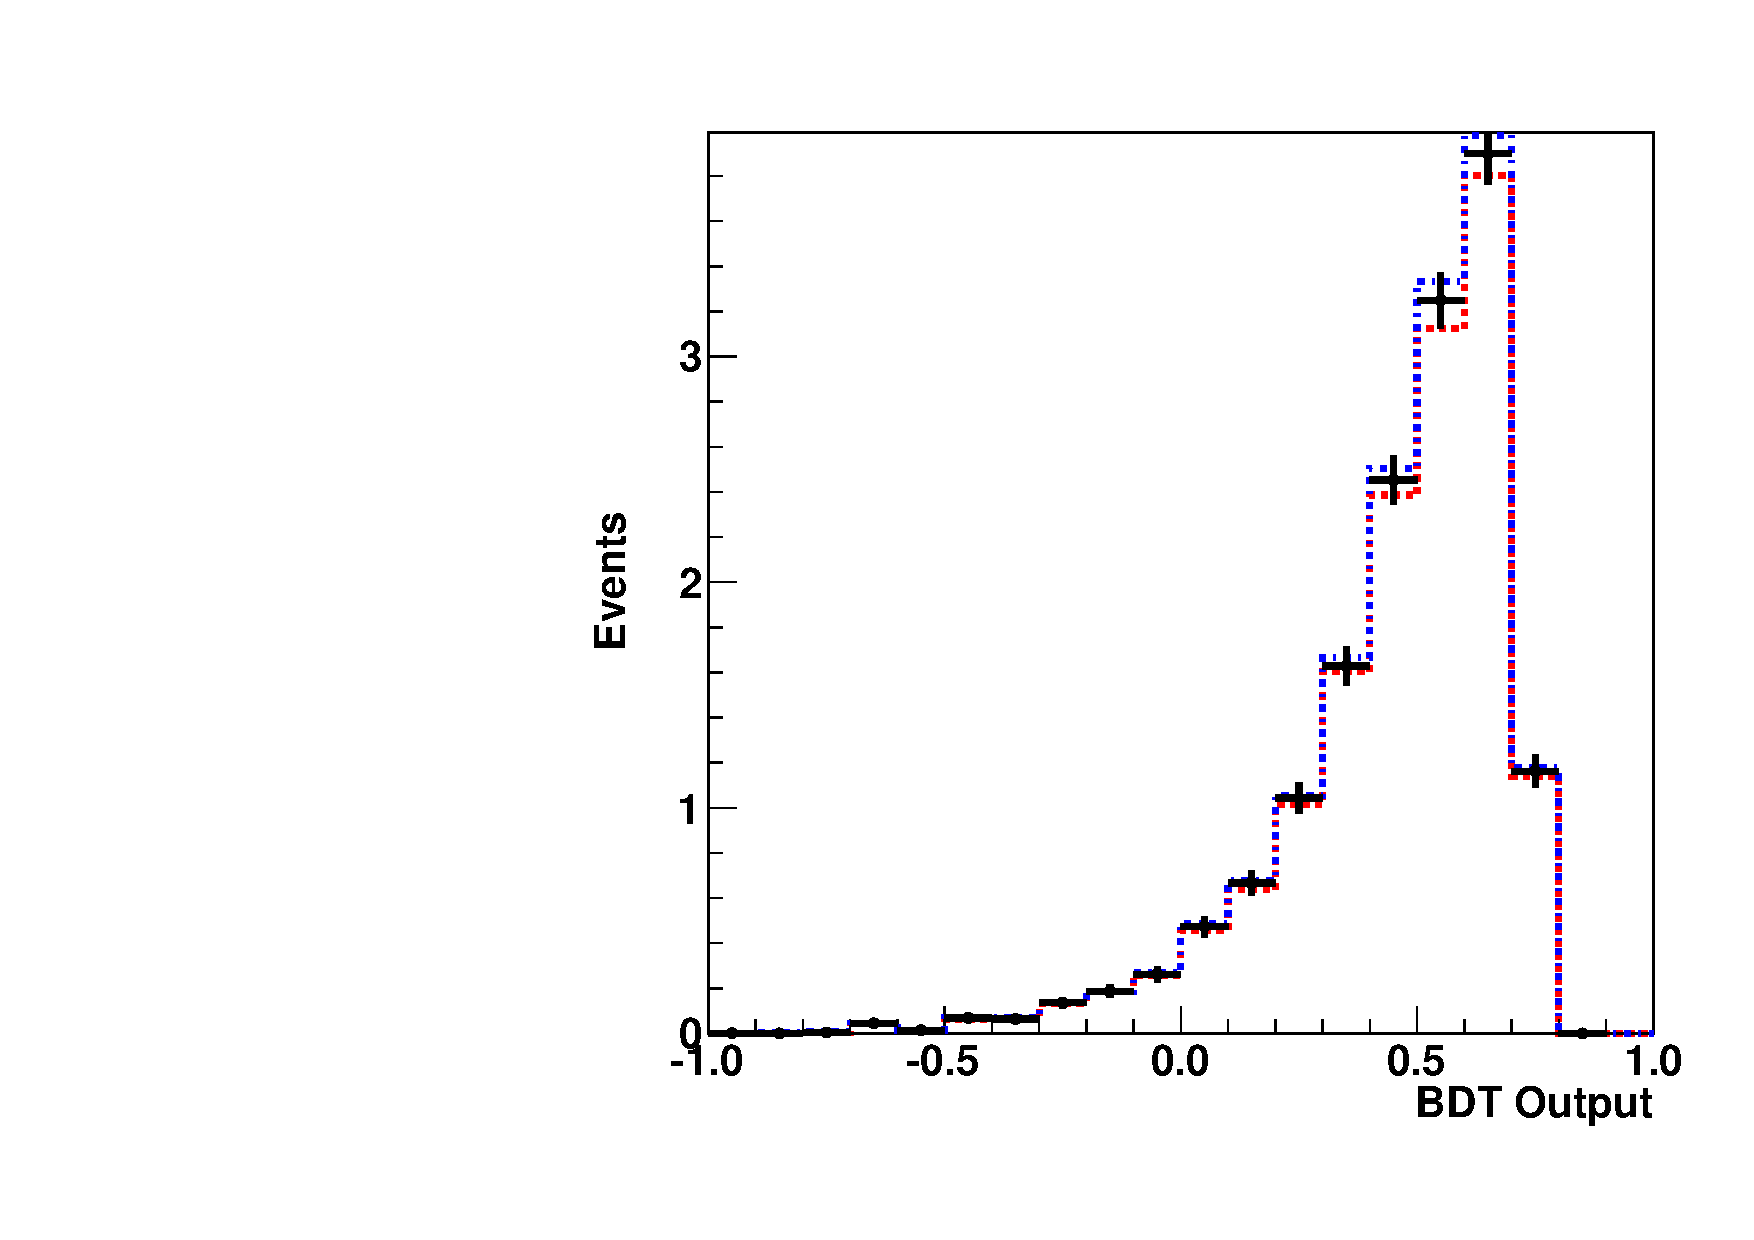
\includegraphics[width=0.49\textwidth]{figures/cvswwsf_50.pdf}}
\caption{BDT Output distribution for $H(130) \to \WW$ 0-jet bin analysis in $gg \to H$ events 
for $\mathcal{L}~=~1.55~\pm~0.07~\ifb$. Opposite-flavor (a) and same-flavor (b) final states 
are shown. The dots histogram is the default shape, while the dashed red histogram 
is the ``Up" component and the dashed blue histograms is the ``Down" component, for the JES 
uncertainties.}
\label{fig:ggHJES}
\end{center}
\end{figure}

\subsubsection{$\WW$ Background}
This effect considers the theoretical uncertainties on the $\WW$ background, in
addition to the normalization uncertainty which has its own factor. The 
$gg \to \WW$ has an uncertainty due to the QCD scales of 50\% and covers very
well any possible shape variation.

To account for possible shape variation on the $qq \to \WW$ process, two 
separate effects are considered. First, we compare the default simulated events
produced with Madgraph generator with simulated events produced with MC@NLO
generator, and this second sample makes the ``up" variation. The ``down"
variation is the mirror of the ratio between both generators. Second, we consider
the uncertainty due to the variation of the QCD scales. To perform that, we take
the ratio between the MC@NLO samples and the ones with the QCD scales up and down. 
An example of the effect of this uncertainty is shown in Figure~\ref{fig:qqWWNorn}. 

\begin{figure}[!htbp]
\begin{center}
\subfigure[]{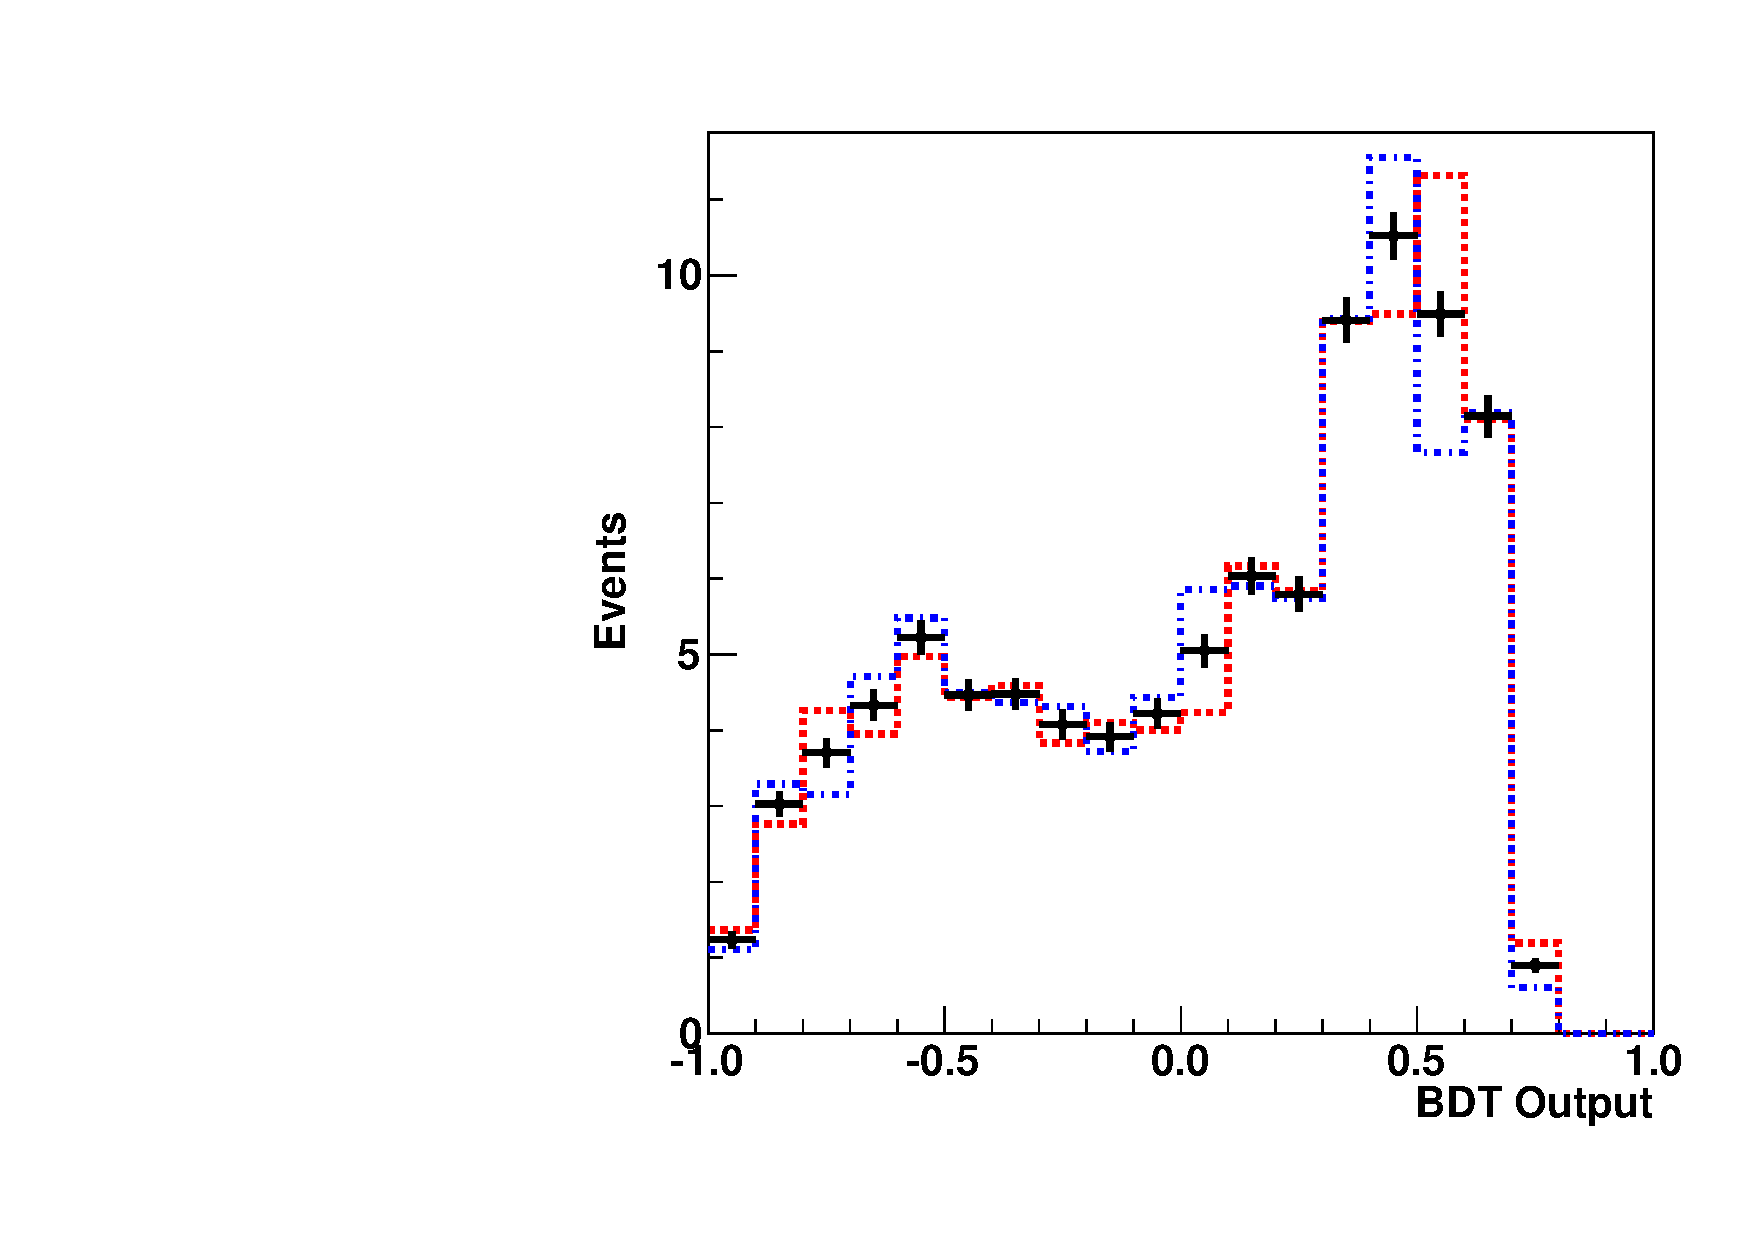
\includegraphics[width=0.49\textwidth]{figures/cvswwof_0.pdf}}
\subfigure[]{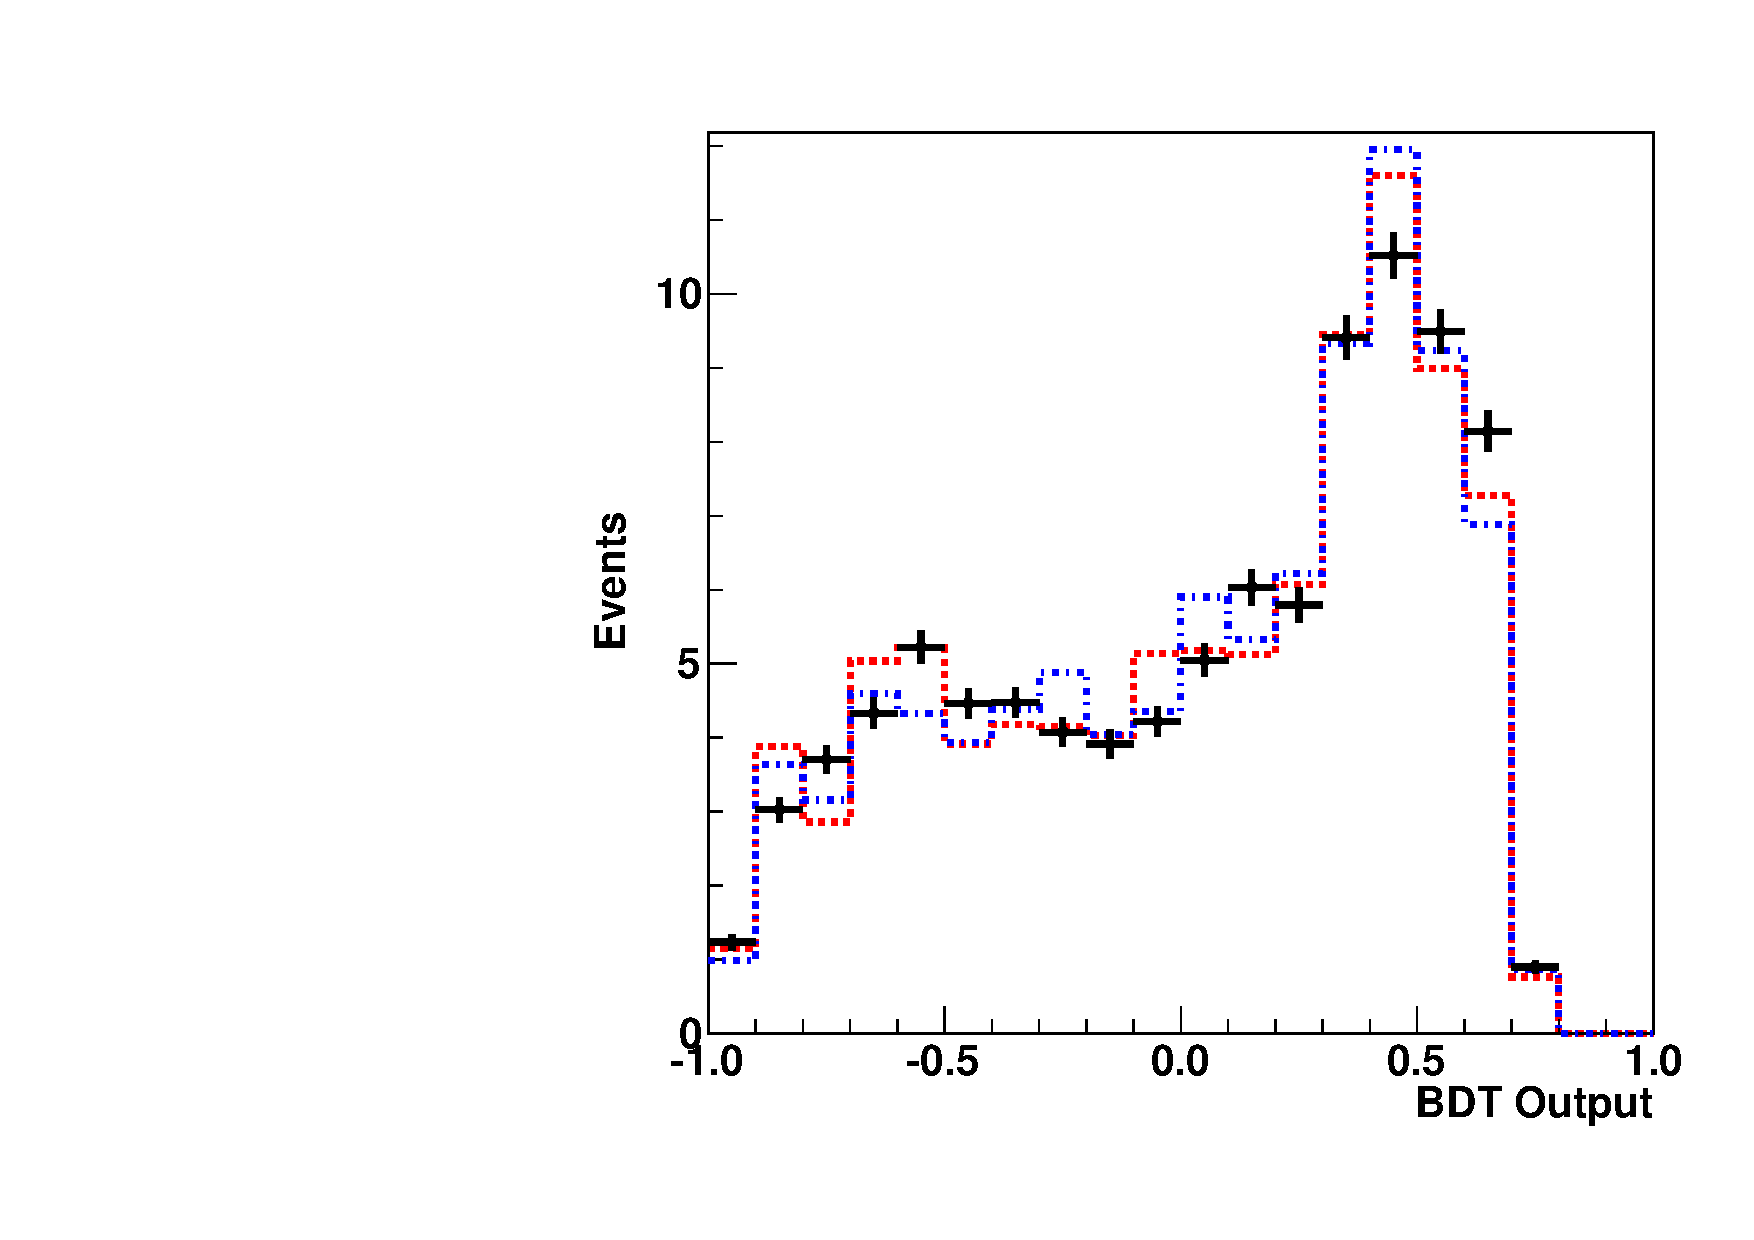
\includegraphics[width=0.49\textwidth]{figures/cvswwof_59.pdf}}
\caption{BDT Output distribution for $H(130) \to \WW$ 0-jet bin analysis opposite-flavor final state in $qq \to \WW$ events 
for $\mathcal{L}~=~1.55~\pm~0.07~\ifb$. The dots histogram is the default shape, while the dashed red histogram 
is the ``Up" component and the dashed blue histograms is the ``Down" component, for the generator 
dependence uncertainty (a) and for the QCD scale uncertainties (b).}
\label{fig:qqWWNorn}
\end{center}
\end{figure}

\subsubsection{$\Wjets$ Background}
The uncertainty due to the $\Wjets$ normalization is as large as $\sim$36\%.
Nevertheless, we may have an additional uncertainty on the shape of the
discriminant variable. Two sources are considered. First, we produce new
distributions by using different lepton fake rates, this is the ``up" variation.
The ``down" variation is the mirror of the ratio between the ``up" and default
distributions. The muon fake rate is built using a jet $\pt$ threshold of 30
$\GeVc$ (instead of 15, the default value), and the electron fake rate is build
using a jet $\pt$ threshold of 50 $\GeVc$ (instead of 35, the default value).
Second, we propagate the Monte Carlo closure test uncertainty. To do that, we use
the lepton plus fakeable object sample from Monte Carlo events and apply 
the measured lepton fake rates to build a new $\Wjets$ distribution. This
produces the ``up" variation. The ``down" variation is the mirror of the ration
between the ``up" and default distributions. 
An example of the effect of this uncertainty is shown in Figure~\ref{fig:WJetsNorn}. 

\begin{figure}[!htbp]
\begin{center}
\subfigure[]{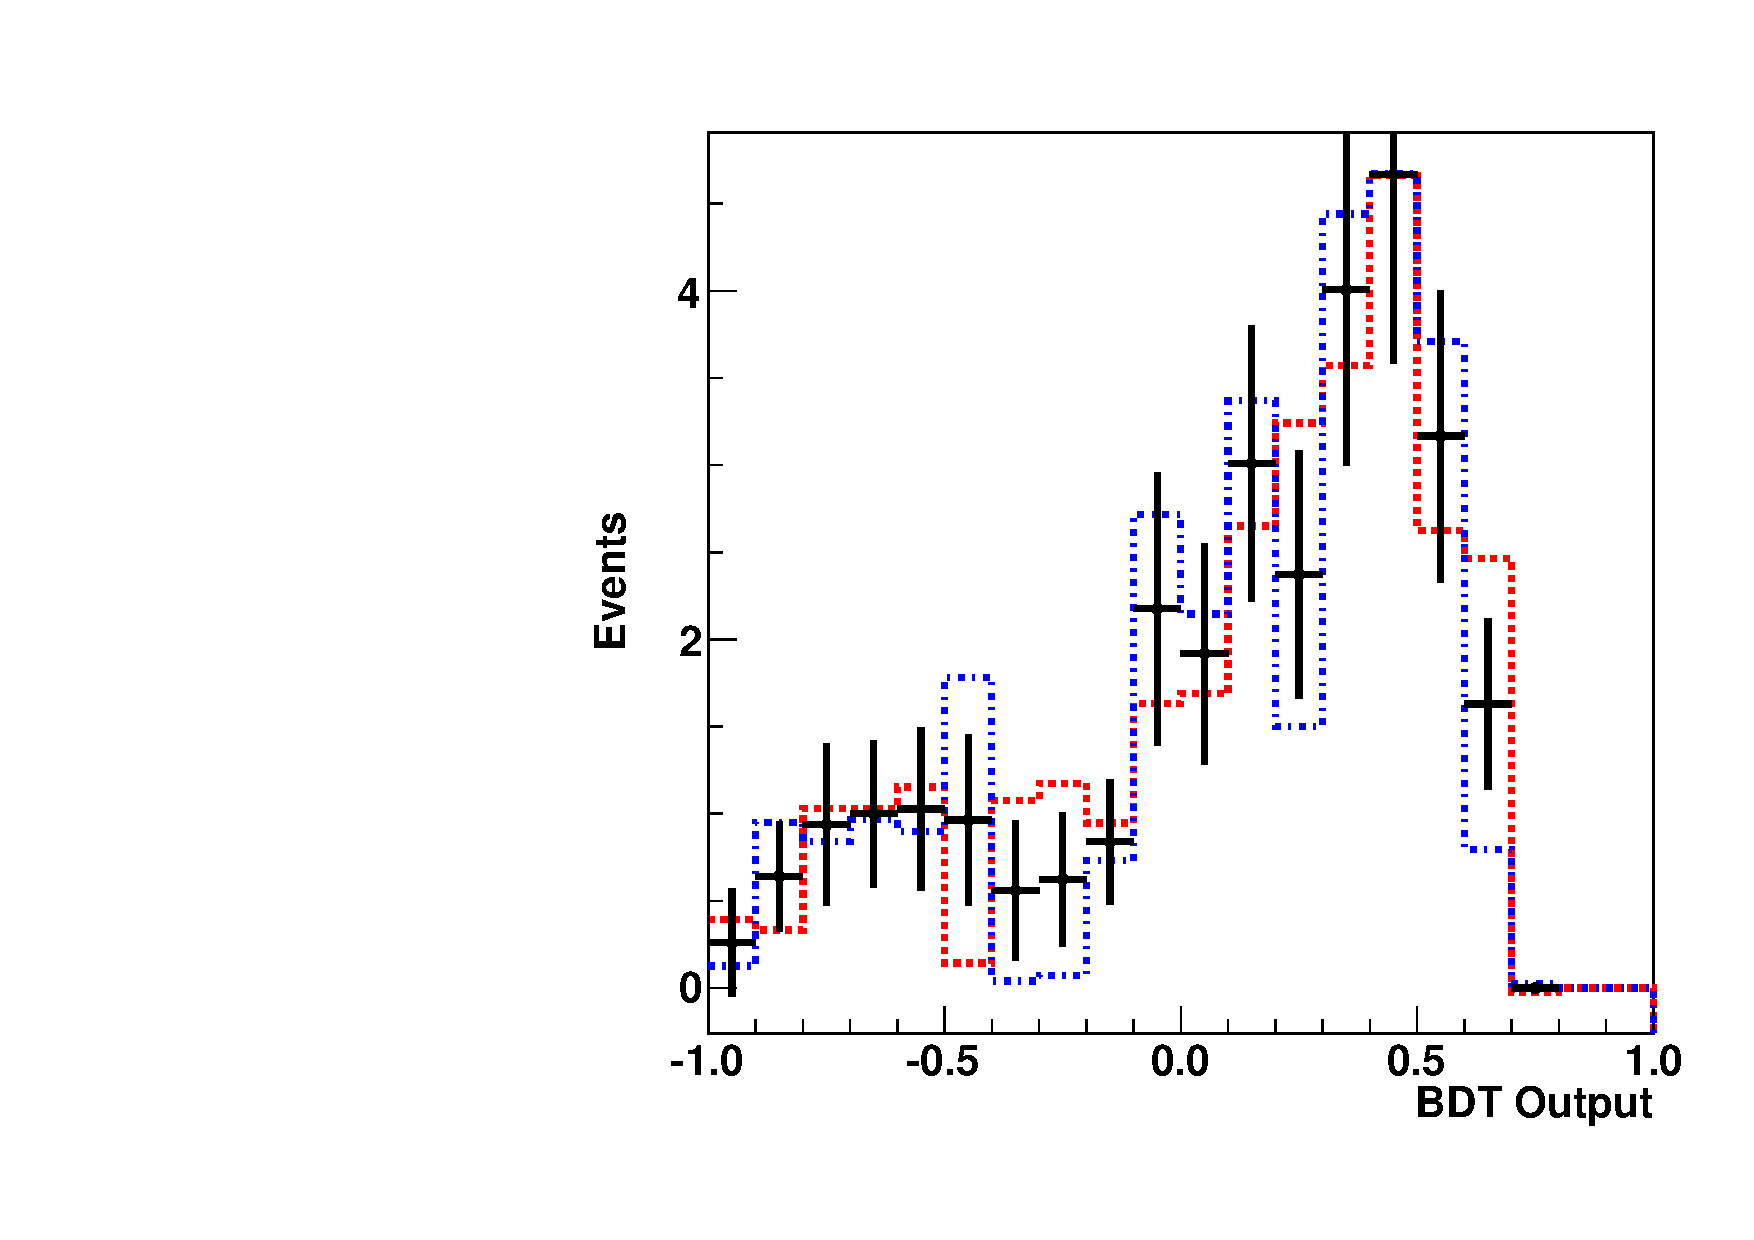
\includegraphics[width=0.49\textwidth]{figures/cvswwof_56.pdf}}
\subfigure[]{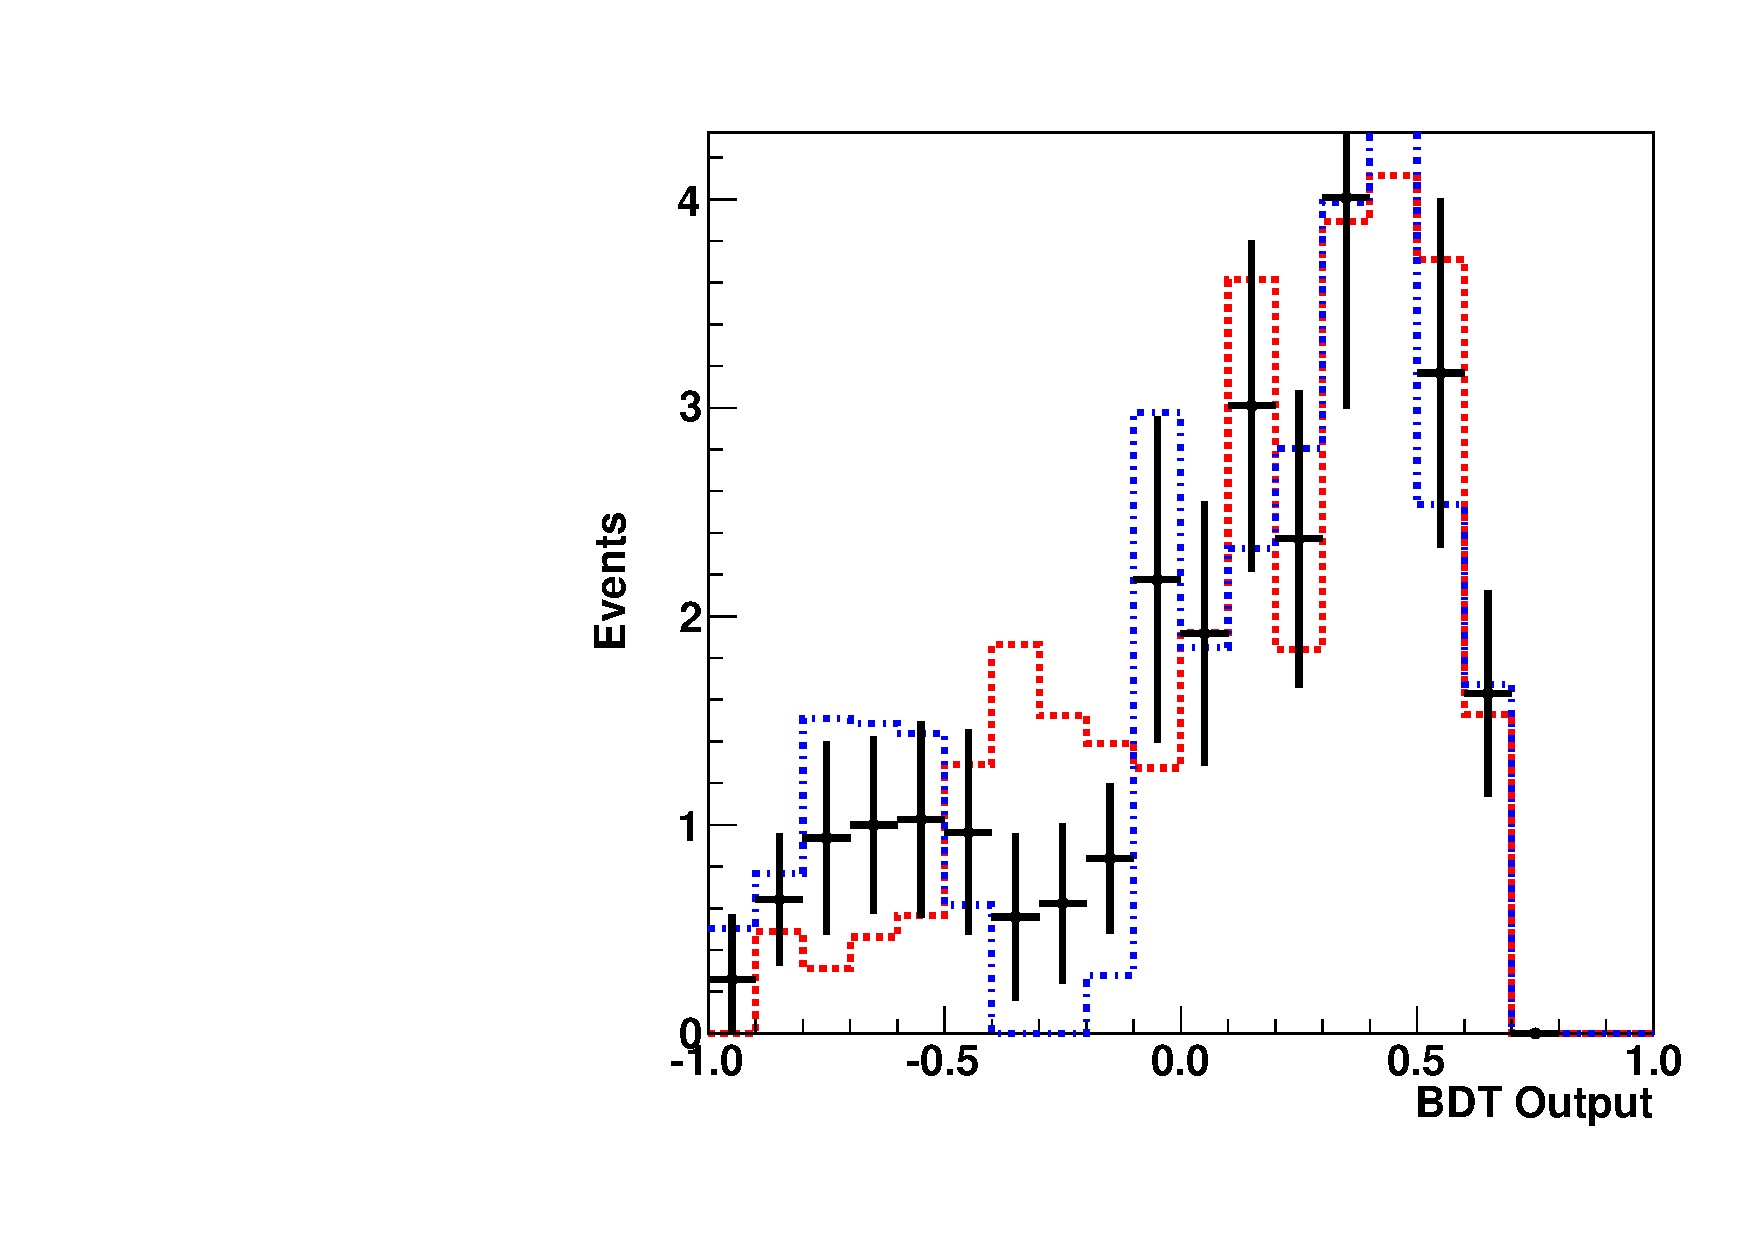
\includegraphics[width=0.49\textwidth]{figures/cvswwof_57.pdf}}
\caption{BDT Output distribution for $H(130) \to \WW$ 0-jet bin analysis opposite-flavor 
final state in $\Wjets$ events for $\mathcal{L}~=~1.55~\pm~0.07~\ifb$. The dots histogram 
is the default shape, while the dashed red histogram is the ``Up" component and the dashed 
blue histograms is the ``Down" component, for the fake rate uncertainty (a) and for the 
Monte Carlo closure test uncertainty (b).}
\label{fig:WJetsNorn}
\end{center}
\end{figure}

\subsubsection{$\dymm$ and $\dyee$ Backgrounds}
The uncertainty on the normalization of this background is rather larger, as
discussed in~\cite{hww_eps}, on the other hand a shape uncertainty could also be
important. Since the number of available simulated events after the final
selection is rather small, the default distribution is taken from events which 
pass all other requirements, but with Min(projected $\met$, projected
track-$\met$) between 20 and 40 $\GeV$, with the normalization obtained from the
signal region evaluation. To have a conservative estimate of the
uncertainty, we take the ``up" variation using the simulated events passing all
requirements, while the mirror of the ratio between the ``up" and default
distributions is the ``down" variation. 

\subsubsection{Top Background}
To account for possible shape uncertainties on the modelling of top simulated
events, we compare different simulated samples with respect to the default ones 
to build the ``up" variation, while the mirror of the ratio between the ``up" 
and default distributions is the ``down" variation. In particular, for $\ttbar$
events we use Madgraph simulated events (Powheg is the default generator), while
for the $\tw$ process we use a sample with different matching procedure.
An example of the effect of this uncertainty is shown in Figure~\ref{fig:topNorm}. 

\begin{figure}[!htbp]
\begin{center}
\subfigure[]{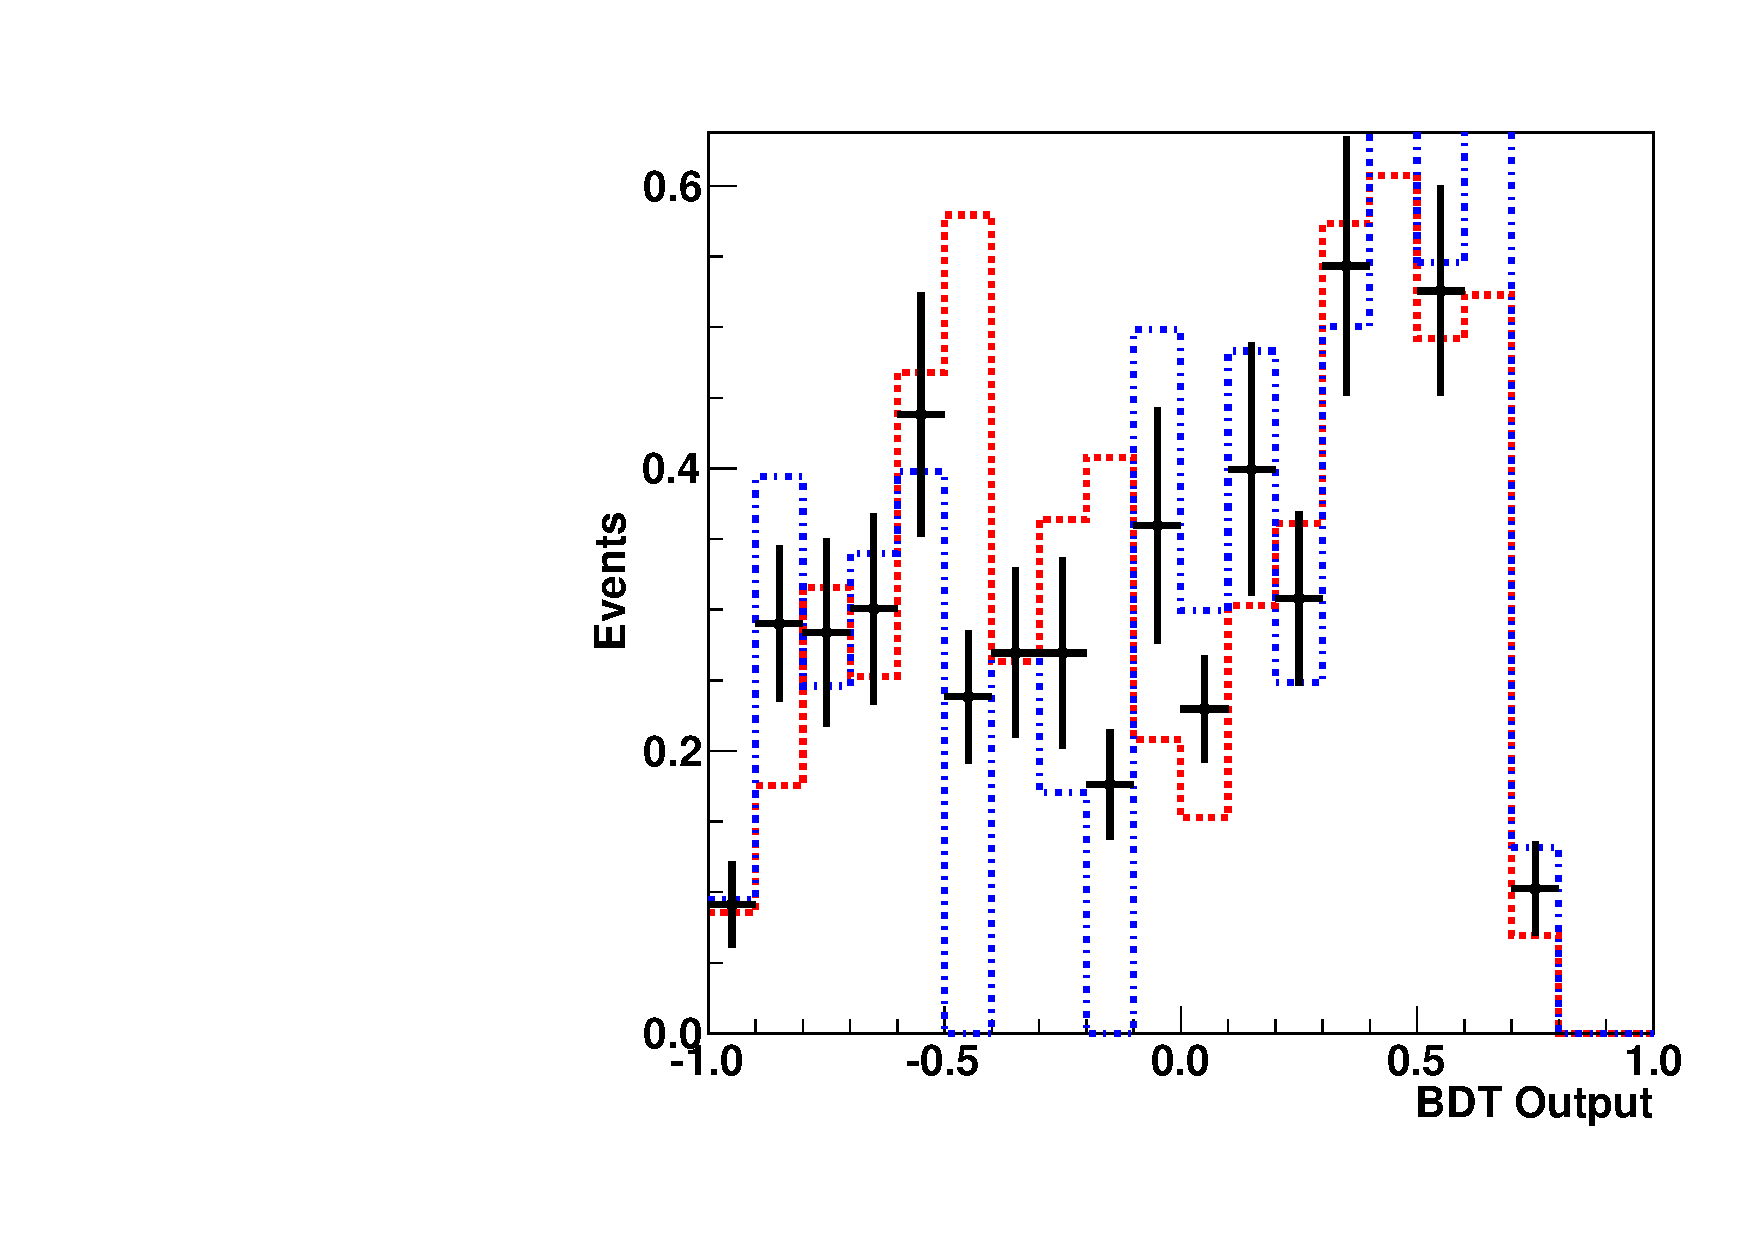
\includegraphics[width=0.49\textwidth]{figures/cvswwof_1.pdf}}
\subfigure[]{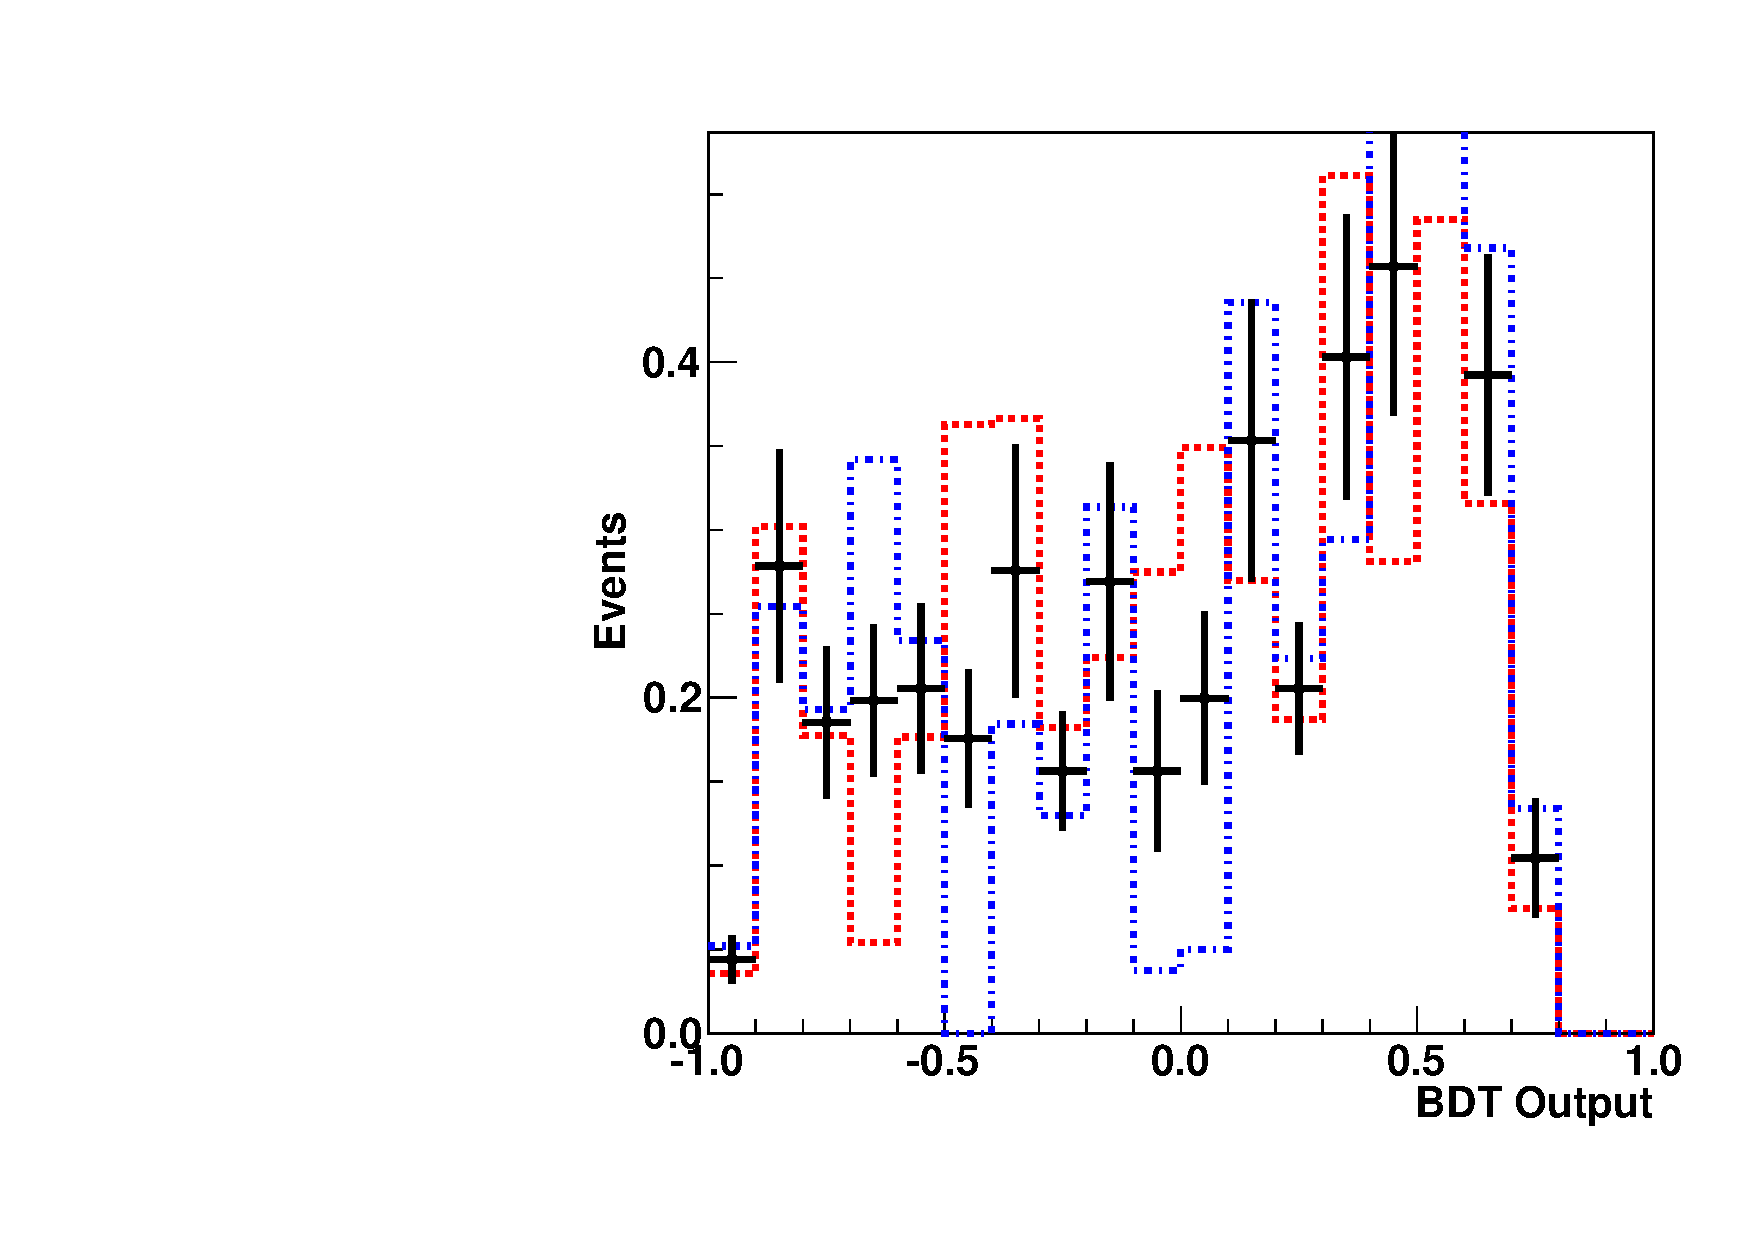
\includegraphics[width=0.49\textwidth]{figures/cvswwsf_1.pdf}}
\caption{BDT Output distribution for $H(130) \to \WW$ 0-jet bin analysis in top events 
for $\mathcal{L}~=~1.55~\pm~0.07~\ifb$. Opposite-flavor (a) and same-flavor (b) final states 
are shown. The dots histogram is the default shape, while the dashed red histogram 
is the ``Up" component and the dashed blue histograms is the ``Down" component, for top 
shape uncertainty.}
\label{fig:topNorm}
\end{center}
\end{figure}

\subsubsection{$\W+\gamma$ Background}
The $\W+\gamma$ background is rather small after our tight preselection
requirements, therefore we do not assign any specific uncertainty due to this
background. The only point to notice is that we take the shape of this process
from a sample of simulated events where the conversion rejection requirements
have been loosened, so that the amount of events used in the final discriminant
variable is larger. We have verified that the shapes do not changed by modifying
those veto requirements within the statistical uncertainties.

\subsubsection{$\dytt$ Background}
The $\dytt$ background is estimated from data using the so-called $\tau$
embedding method. The aim of this method is to create hybrid events with two 
muons (or electrons) coming from a data $\Z$ decay replaced by two 
(simulated) $\tau$ particles. Different techniques for creating such events
exist to replace the muons: either at offline level, at the reconstruction 
level or at the digitazitation level. In addition to the use of data to a very
large extent, this method allows for an increase on the statistical power of the
sample leading to much smaller statistical uncertainties.

\subsubsection{Bin-By-Bin Statistical Uncertainty}
As already stated in Section~\ref{sec:methods}, the current available official 
framework do not support a full proper treatment of the statistical 
uncertainties on each bin independently of the discriminant variable. A way to
account for most of the effect is to build ``up" (``down") variation as the
+1(-1)$\sigma$ statistical uncertainty on every bin. In this way, we properly
consider the uncertainty on every bin, although in a correlated way. 
An example of the effect of this uncertainty is shown in Figure~\ref{fig:qqWWStat}. 

\begin{figure}[!htbp]
\begin{center}
\subfigure[]{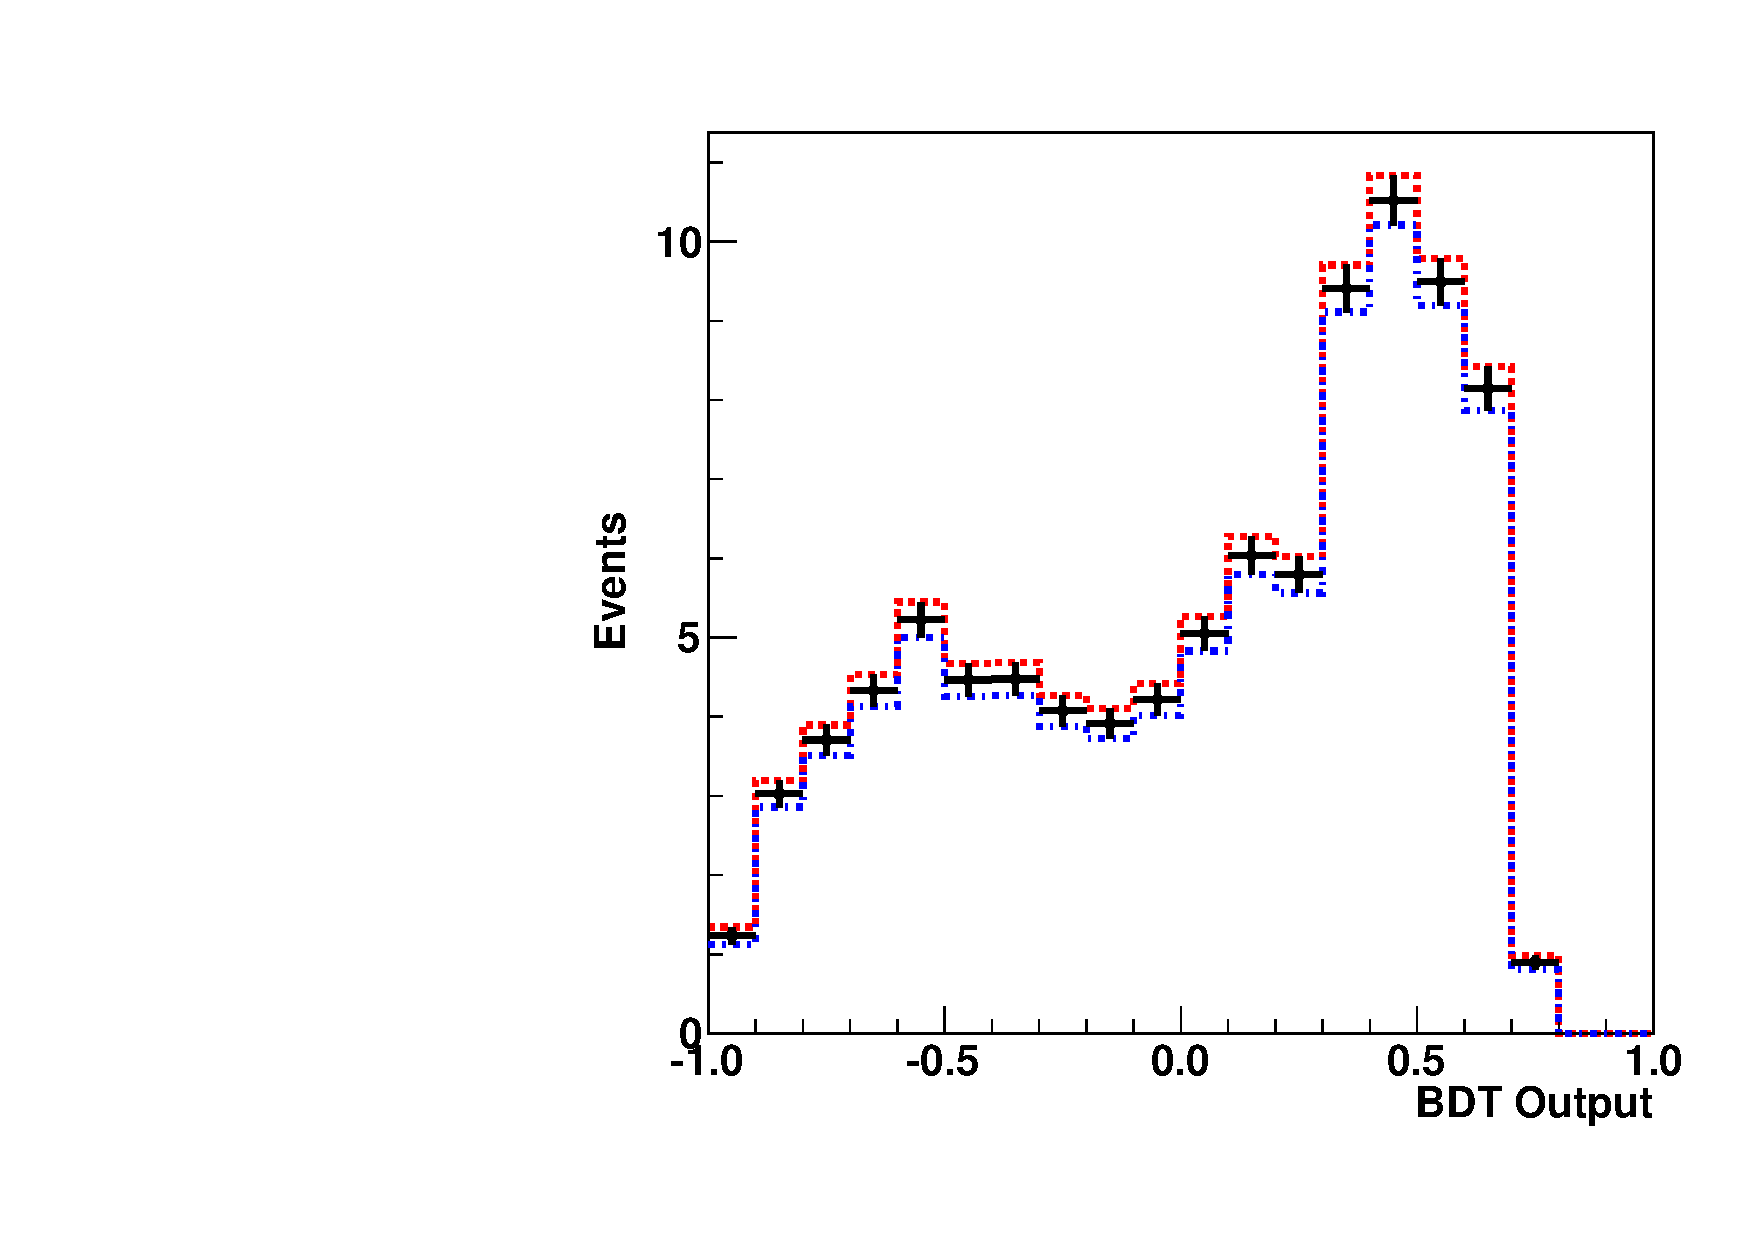
\includegraphics[width=0.49\textwidth]{figures/cvswwof_7.pdf}}
\subfigure[]{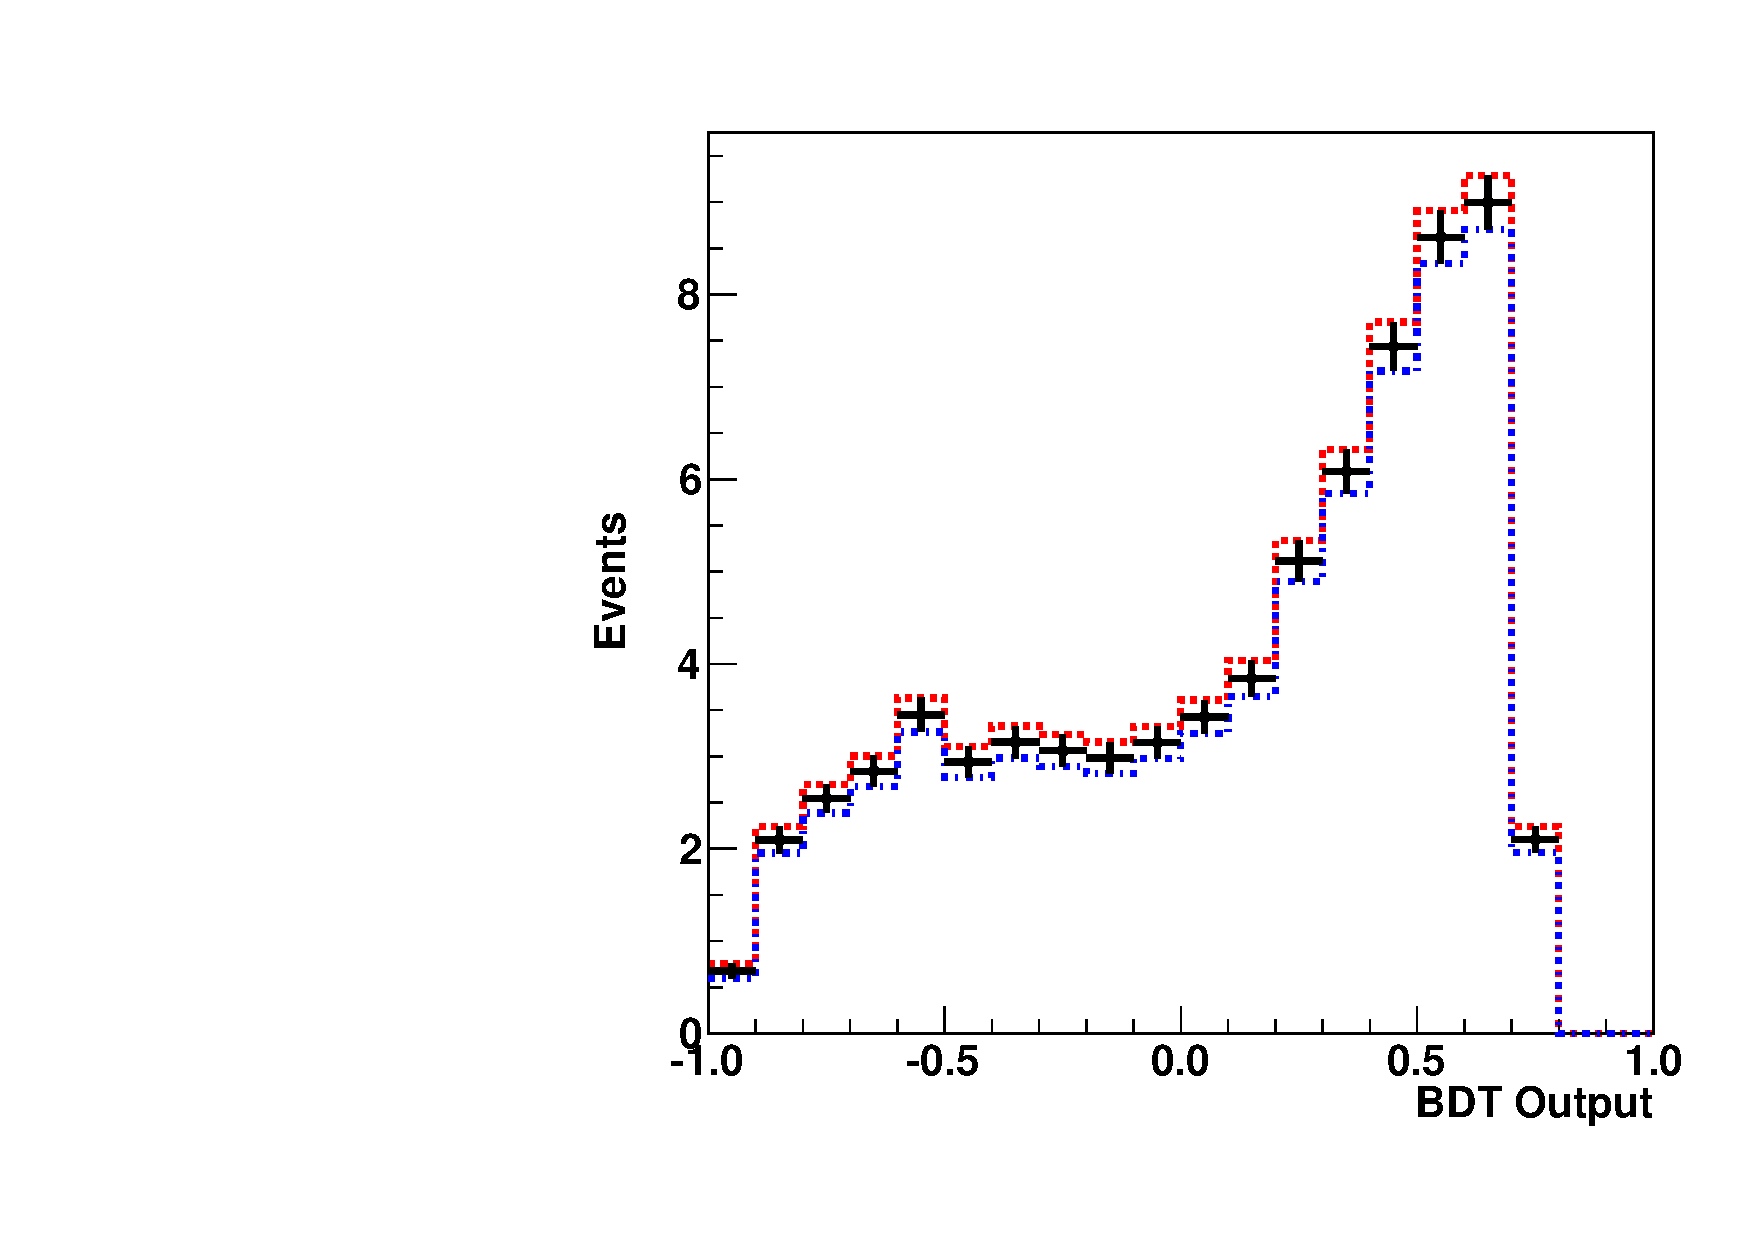
\includegraphics[width=0.49\textwidth]{figures/cvswwsf_7.pdf}}
\caption{BDT Output distribution for $H(130) \to \WW$ 0-jet bin analysis in $qq \to \WW$ events 
for $\mathcal{L}~=~1.55~\pm~0.07~\ifb$. Opposite-flavor (a) and same-flavor (b) final states 
are shown. The dots histogram is the default shape, while the dashed red histogram 
is the ``Up" component and the dashed blue histograms is the ``Down" component, for statistical 
shape uncertainty.}
\label{fig:qqWWStat}
\end{center}
\end{figure}

As a cross-check, we perform the following: (a) we divide the discriminant
variable into 3 regions (low, medium, and high values), (b) for the ``up" 
variation we move all low points up by one $\sigma$ and all high points down 
by one $\sigma$, (c) for the "down" variation we do the opposite. With this
procedure we create an artificial shape variation due to the statistical
uncertainties. It is a conservative approach, but it gives an idea of the size of
the effect. 
An example of the effect of this uncertainty is shown in Figure~\ref{fig:qqWWStatAlt}. 

\begin{figure}[!htbp]
\begin{center}
\subfigure[]{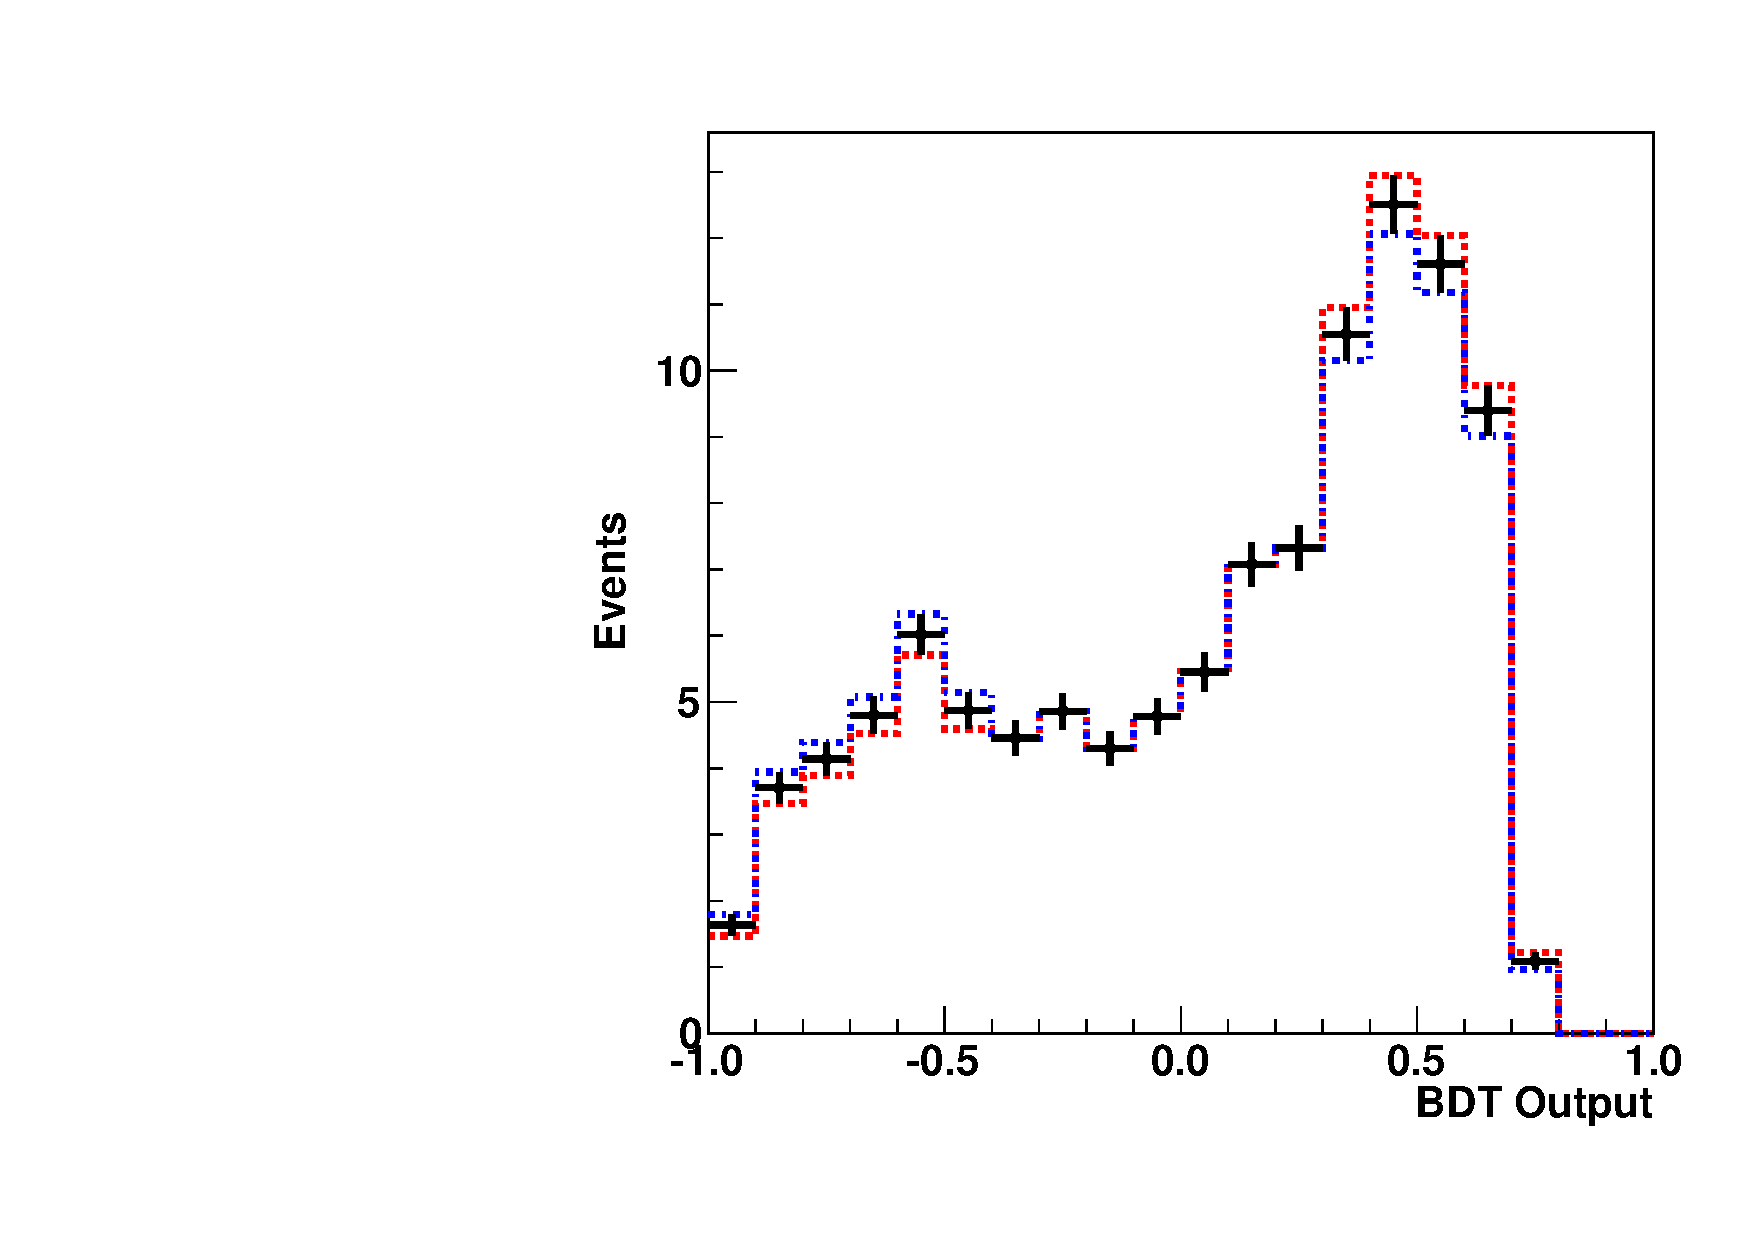
\includegraphics[width=0.49\textwidth]{figures/cvswwof_7_alt.pdf}}
\subfigure[]{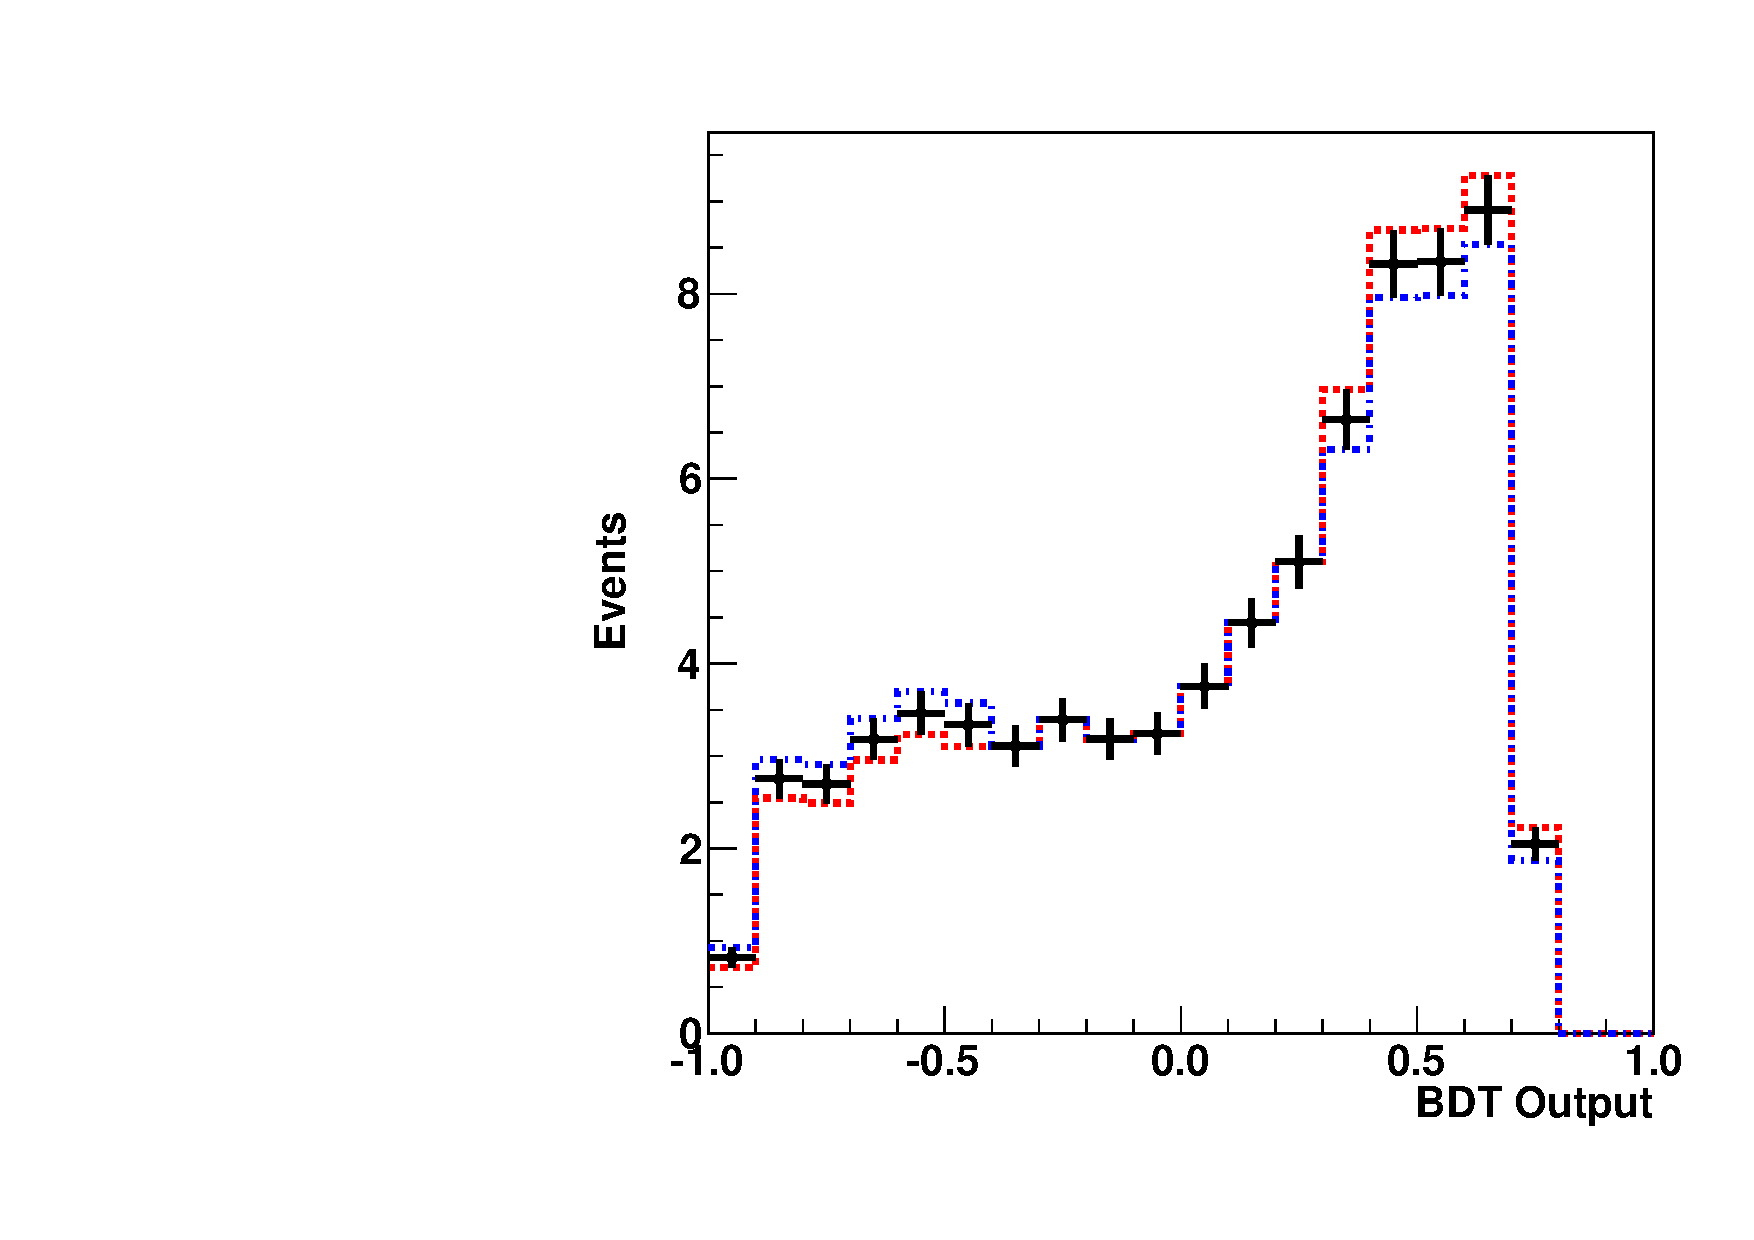
\includegraphics[width=0.49\textwidth]{figures/cvswwsf_7_alt.pdf}}
\caption{BDT Output distribution for $H(130) \to \WW$ 0-jet bin analysis in $qq \to \WW$ events 
for $\mathcal{L}~=~1.55~\pm~0.07~\ifb$. Opposite-flavor (a) and same-flavor (b) final states 
are shown. The dots histogram is the default shape, while the dashed red histogram 
is the ``Up" component and the dashed blue histograms is the ``Down" component, for statistical 
shape uncertainty using an alternative approach.}
\label{fig:qqWWStatAlt}
\end{center}
\end{figure}
